\documentclass[
11pt, % The default document font size, options: 10pt, 11pt, 12pt
%oneside, % Two side (alternating margins) for binding by default, uncomment to switch to one side
english, % ngerman for German
onehalfspacing, % Single line spacing, alternatives: onehalfspacing or doublespacing
%draft, % Uncomment to enable draft mode (no pictures, no links, overfull hboxes indicated)
%nolistspacing, % If the document is onehalfspacing or doublespacing, uncomment this to set spacing in lists to single
%liststotoc, % Uncomment to add the list of figures/tables/etc to the table of contents
%toctotoc, % Uncomment to add the main table of contents to the table of contents
parskip, % Uncomment to add space between paragraphs
%nohyperref, % Uncomment to not load the hyperref package
headsepline, % Uncomment to get a line under the header
%chapterinoneline, % Uncomment to place the chapter title next to the number on one line
%consistentlayout, % Uncomment to change the layout of the declaration, abstract and acknowledgements pages to match the default layout
]{MastersDoctoralThesis} % The class file specifying the document structure
\usepackage[utf8]{inputenc} % Required for inputting international characters
\usepackage{csquotes}
\usepackage[T1]{fontenc} % Output font encoding for international characters
\usepackage{mathpazo} % Use the Palatino font by default
\usepackage{blindtext}
\usepackage{amsmath}
\usepackage{mathtools}
\usepackage{amssymb}
\usepackage[toc,page]{appendix}
\usepackage{tablefootnote}
\usepackage[sorting=none, maxnames=99]{biblatex}
\addbibresource{bibliography.bib} % The filename of the bibliography
\usepackage{graphicx}   % For including images
\usepackage{subcaption} % For subfigures

\usepackage{circuitikz}
\usepackage{tikz}
%\usepackage{svg}
\usetikzlibrary{shapes.geometric, decorations.pathmorphing, positioning}
\usepackage{float}
%\usepackage[autostyle=true]{csquotes} % Required to generate language-dependent quotes in the bibliography

%----------------------------------------------------------------------------------------
%	MARGIN SETTINGS
%----------------------------------------------------------------------------------------

\geometry{
	paper=a4paper, % Change to letterpaper for US letter
	inner=2.5cm, % Inner margin
	outer=3.8cm, % Outer margin
	bindingoffset=.5cm, % Binding offset
	top=1.5cm, % Top margin
	bottom=1.5cm, % Bottom margin
	%showframe, % Uncomment to show how the type block is set on the page
}


% ------------------------------------------
%      MY PACKAGES
% ------------------------------------------
\usepackage{bookmark}
\usepackage{todonotes}
\usepackage[inkscapelatex=false]{svg}
\usepackage{amsmath}
\usepackage{amsthm}
\usepackage{comment}
\usepackage{skull}
\usepackage{amsmath}
\usepackage{algorithm}
\usepackage{algpseudocode}
\usepackage{svg}

% theorems
\newtheorem{theorem}{Theorem}
\newtheorem{definition}{Definition}
\newtheorem{lemma}{Lemma}
\newtheorem{corollary}{Corollary}
\newtheorem{proposition}{Proposition}
\newtheorem*{remark}{Remark}

\addbibresource{bibliography.bib} % The filename of the bibliography


\newcommand{\gnote}[1]{\todo[inline, color=green!40]{#1}}
\newcommand{\onote}[1]{\todo[inline, color=orange]{#1}}
\newcommand{\mol}{\mathcal{M}}
\newcommand{\xb}{\mathbf{x}}
\newcommand{\norm}[1]{\lVert {#1} \rVert}
\DeclareMathOperator*{\argmax}{arg\,max}
\DeclareMathOperator*{\argmin}{arg\,min}

\usepackage{color, colortbl}
\definecolor{LightGrey}{rgb}{0.88,0.88,1}
\definecolor{LightGreen}{rgb}{0.88,1,0.88}
\definecolor{LightRed}{rgb}{1,0.88,0.88}

\thesistitle{Exploring Deep Reservoir Computing with structured modular architectures} % Your thesis title, this is used in the title and abstract, print it elsewhere with \ttitle
\supervisor{Prof. Claudio Gallicchio\\Dott. Andrea Ceni\\Dott. Andrea Cossu, } % Your supervisor's name, this is used in the title page, print it elsewhere with \supname
\examiner{} % Your examiner's name, this is not currently used anywhere in the template, print it elsewhere with \examname
\degree{Master's Degree} % Your degree name, this is used in the title page and abstract, print it elsewhere with \degreename
\author{Vincenzo Gargano} % Your name, this is used in the title page and abstract, print it elsewhere with \authorname
\addresses{} % Your address, this is not currently used anywhere in the template, print it elsewhere with \addressname

\subject{Computer Science} % Your subject area, this is not currently used anywhere in the template, print it elsewhere with \subjectname
\keywords{} % Keywords for your thesis, this is not currently used anywhere in the template, print it elsewhere with \keywordnames
\university{Università di Pisa} % Your university's name and URL, this is used in the title page and abstract, print it elsewhere with \univname
\department{Department of Computer Science} % Your department's name and URL, this is used in the title page and abstract, print it elsewhere with \deptname
%group{\href{http://researchgroup.university.com}{Research Group Name}} % Your research group's name and URL, this is used in the title page, print it elsewhere with \groupname
%\faculty{\href{http://faculty.university.com}{Faculty Name}} % Your faculty's name and URL, this is used in the title page and abstract, print it elsewhere with \facname

\AtBeginDocument{
\hypersetup{pdftitle=\ttitle} % Set the PDF's title to your title
\hypersetup{pdfauthor=\authorname} % Set the PDF's author to your name
\hypersetup{pdfkeywords=\keywordnames} % Set the PDF's keywords to your keywords
}

\begin{document}

%%%% TITLE

\begin{titlepage}
	\begin{center}
		% maybe change it
		\includegraphics[width=0.6\textwidth]{assets/cherubino_black.eps} \\
		\vspace*{.06\textheight}
		%{\scshape\LARGE \univname\par}
		\vspace{0.5cm} % University name
		\textsc{\Large Master's Degree Thesis}\\[0.5cm] % Thesis type

		\Large \textit{Dipartimento di Informatica \\ Corso di Laurea Magistrale in Informatica}\\[1cm] % University requirement text

		\HRule \\[0.4cm] % Horizontal line
		{\huge \bfseries \ttitle\par}\vspace{0.4cm} % Thesis title
		\HRule \\[1.5cm] % Horizontal line

		\begin{minipage}[t]{0.4\textwidth}
			\begin{flushleft} \large
				\emph{Author:}\\
				\authorname % Author name - remove the \href bracket to remove the link
			\end{flushleft}
		\end{minipage}
		\begin{minipage}[t]{0.4\textwidth}
			\begin{flushright} \large
				\emph{Supervisors:} \\
				\supname % Supervisor name - remove the \href bracket to remove the link
			\end{flushright}
		\end{minipage}\\[3cm]

		\vfill
		%\groupname\\\deptname\\[2cm] % Research group name and department name

		\vfill

		Academic Year 2024/2025\\[4cm] % Date
		%\includegraphics{Logo} % University/department logo - uncomment to place it

		\vfill
	\end{center}
\end{titlepage}


\section*{}
\thispagestyle{empty}
\vfill
\begin{center}
	\Large \textbf{Abstract}
	\\[0.5cm]
	\normalsize
% Enter abstract of your thesis here, this will appear on the title page
(Da rivedere è solo un draft)
In this work, we present two novel architectures, Deep Cycle Echo State Network (DeepCycleESN) and Deep Antisymmetric Echo State Networks (DeepAntisymESN) in the field of Reservoir Computing (RC). By changing the usual deep hierarchical setting to a structured one that relies on information flow across networks.
Subsequentily we extend these structured modularities to a promising RC model: Recurrent Oscillator Networks (RON), which offer a richer dynamical pool than simple ESNs.
 Both novel architectures are inspired by recent advances in the RC field and use deep-layer construction with 
 a structured modular topology.
 We evaluate the proposed models on several benchmark tests for RC, showing that they are able to
 outperform on memory capacity and long-term prediction tasks by comparing state-of-the-art shallow and deep RC architectures.
 We briefly analyse their linearized behaviour in order to
 provide insights into the role of modularity and depth in RC.
\end{center}

\vfill
%\hypersetup{linkcolor=red}
{
	\hypersetup{linkcolor=purple!30!black, linktoc=all}
	\tableofcontents
}


\chapter{Introduction}\label{ch:introduction}
\section{Motivation and Objectives}
\todo{Forse dovrei concentrarmi più su RNN dall'inizio?}
Nowadays, Artificial Intelligence (AI) became the main driver of innovation in many fields, at the point that the growth of research
became exponential in the last decade. This fully alignes with the current state of our world, in fact,
we are observing a paradigm shift in the way we interact with technology (or world), through the use of AI.\newline
Within AI, whose main goal is not only to understand \textit{intelligence}, but to embed it into agents capable of performing complex tasks through
\textit{rational reasoning, planning} and \textit{acting}, the subfield of Machine Learning (ML) has emerged as the dominant approach to mimicking biological intelligent behaviour.
Neural Networks (NN) \textit{learn} complex patterns from large amounts of real-world data, instead of relying on explicit rule based approaches,
in order to perform \textit{inference} and return prediction on unseen data. \newline
The last years have seen a surge in popularity of generative models, after a first wave of discriminative models that made popular the field of Deep Learning (DL),
and introduced GPU computation in 2009 \cite{Raina2009LSDL}. 
Particularly, deep generative models have been applied with unbelievable results in many fields,
 from image generation with \textit{Diffusion Models} \cite{ho2020denoisingdiffusionprobabilisticmodels}
 to text generation with \textit{Transformers} \cite{vaswani2023attentionneed} and protein folding with
\textit{Alphafold} \cite{jumper2021highly} and many others domains, achieving state of the art results.
However, deep learning models are known to be expensive in both training and inference, requiring large 
amount of computational resources (GPU production) and energy consumption \cite{article}.

\section{Reservoir Computing for Efficient AI} \todo{mancano citazioni ed è ripetitivo rispetto al background}
Sequential data processing remains a fundamental challenge in machine learning, from natural language to time series forecasting.
While Recurrent Neural Networks (RNNs) have been the traditional approach for modeling temporal dependencies, 
training them to capture long-term patterns has proven notoriously difficult due to vanishing and exploding gradients.
Although architectures like LSTMs and GRUs have partially addressed these issues through gating mechanisms,
and Transformers have recently dominated the field with their attention-based approach, these solutions come at the cost
of increased architectural complexity and computational demands.\newline
An alternative paradigm that has gained attention is Reservoir Computing (RC)\cite{}, which offers a fundamentally different approach
to sequential processing. By maintaining a fixed, randomly initialized recurrent network as a "reservoir" of dynamics,
and training only a simple linear readout layer, RC circumvents the gradient-based training of recurrent connections entirely.
This framework not only simplifies the learning process but also draws inspiration from neuroscience and physical computing systems,
where rich dynamics emerge naturally without explicit optimization.\newline

Despite its computational efficiency and theoretical elegance, vanilla RC models face their own set of limitations,
particularly in scaling to complex tasks that require multiple levels of temporal abstraction\cite{}.
This motivates the exploration of \textit{deep} variants \cite{} of reservoir computing architectures,
which aim to combine the efficiency of the RC paradigm with the representational power of hierarchical processing.
This thesis investigates such deep reservoir architectures, examining how stacking multiple reservoir layers
can enable learning at different timescales while maintaining the training efficiency that makes RC attractive.\newline


\section{Scientific contribuition}
\todo{After finishing experimental part...}


\section{Structure of the work}

elenco puntato con quello che si dirà in ogni capitolo della tesi

\chapter{Background}\label{ch:background}

In this chapter we will review the main concepts and theory needed to understand the rest of this thesis.
We will start with a brief introduction of the Dynamical Systems (DS) theory and an overview of Machine Learning
concepts and foundational models that will be useful to understand the rest of the work.
%Then we will move to a more specific topic, about RC and the ESN model, 
%with some enphasis on the Deep counterparts of both models treated in this work.


\section{The Inherent Dynamism of Natural Systems}\todo{questo va nel background}
Our universe is essentially a complex non-linear dynamical system, and since Newton in mid 1600s, used differential equations as a method
to solve the two body problems, but many natural phenomena are essentially Complex Systems, from small components of the 
environment there are interdependaces \todo{devo approfondire i sistemi complessi?} (CS) which exhibit dynamics that evolve through time:
such as motion of planets, flow of fluids, weather changes, growth of population and many others phenomena.\newline

Dynamics is a fundamental piece of reality and modeling time dependent system evolution, is crucial to understand the world around us:
eg. the design of control system, stock market and also the human brain can be modeled as a dynamical system.
\todo{forse questa parte sui framework non va messa qui} The methodological framework developed through the preceding century have been specifically designed to analyze sequential data structures, commonly referred as \textit{time series},
These approaches encompass techniques such as Autoregressive (AR) 
models (i should cite but cannot find source) which employ linear regression on data sequences,
extending to more sophisticasted frameworks including State-Space Models \cite{kalman1960new}, originally developed for Control Theory applications,
 and Hidden Markov Models (HMM) \cite{baum1966statistical}. The latter served as fundational precursors to Recurrent Neural Netowrks \cite{ELMAN1990179} (RNNs).
 The aforementioned models, are the basis of modern neural based sequential modeling.\newline


\section{Dynamical Systems review}
A dynamical system is a system which evolves over time, we can describe it's changes throught \textbf{state variables}, usually many models are constructed such that
only the foundamental state variables are considered, for example \textit{biological spiking neurons} modeled as in \cite{1257420} are described by a simple 2-D dimensional ODE, where the two state variables are the membrane potential and a recovery variable.
ignoring existing other possible variables such gradient of ion concentration, temperature; for the sake of obtaining a large scale simulation.\newline

There are two types of dynamical systems: \textit{Differential Equations}, which are continuous in time,
and Difference Equations or \textit{Iterated Maps} which are discrete in time. 
The most used in a wide range of sciences fields are the former, which are further distinguished in Ordinary Differential Equations (ODE) 
and Partial Differential Equations (PDE), the difference is that in PDE we have two or more independent variables.  \newline

This thesis will focus on ODEs since our models fell into that category, but we will also use \textit{discretization methods} (link to the section maybe) to obtain it's approximated solution.\newline
 Formally we define an ODE as:
\begin{equation}
    \frac{d\mathbf{x}}{dt} = f(\mathbf{x},t)
\end{equation}
where $\mathbf{x} \in \mathbb{R}^n$ is the state vector, $t$ is the time and $f:\mathbb{R}^n \times \mathbb{R} \rightarrow \mathbb{R}^n$ is a
vector field grouping all the state variables that describe the evolution of the system. \newline

\todo{questo va tolto, forse è meglio non andare troppo in dettaglio con queste cose}
An example of ODE is the well known Dampened Harmonic Oscillator:
\begin{equation} \label{eq:armonic}
    \frac{d^2x}{dt^2} + 2\beta \frac{dx}{dt} + \omega_0^2 x = 0
\end{equation}
where $x$ is the position of the oscillator, $\beta$ is the damping coefficient and $\omega_0$ is the natural frequency of the oscillator.
\todo{anche questo va tolto?}

A Differential Equation is \textit{autonomous} if the function $f$ does not depend explicitly on time, otherwise is \textit{non-autonomous}.
We can switch from a non-autonomous to an autonomous system by adding time as a new variable to the state vector, for example the
non-autonomous system of equation \ref{eq:armonic} can be rewritten with a change of variable.

\clearpage
\subsection{Modeling}
Modeling is a central methodology in the study of complex systems, translating real world observations and hypoteses into a formalized mathematical model, even tough simplified, can be
crucial for studying emergent behaviours, particlarly in natural systems where we cannot change the initial state, or the enviroment variables that influence it.
\newline
The Hodgkin-Huxley model \cite{hodgkin1952quantitative} describes the dynamics of neuronal membrane
potential through an equivalent electrical circuit. The membrane can be represented as a capacitor $C_m$ 
in parallel with several ion channels, each modeled as a voltage-dependent conductance 
in series with a battery representing the ion's reversal potential.
\newline
\begin{figure}[H]
    \centering
    \begin{tabular}{m{0.35\textwidth}@{\hspace{1cm}}c@{\hspace{1cm}}m{0.45\textwidth}}
        \centering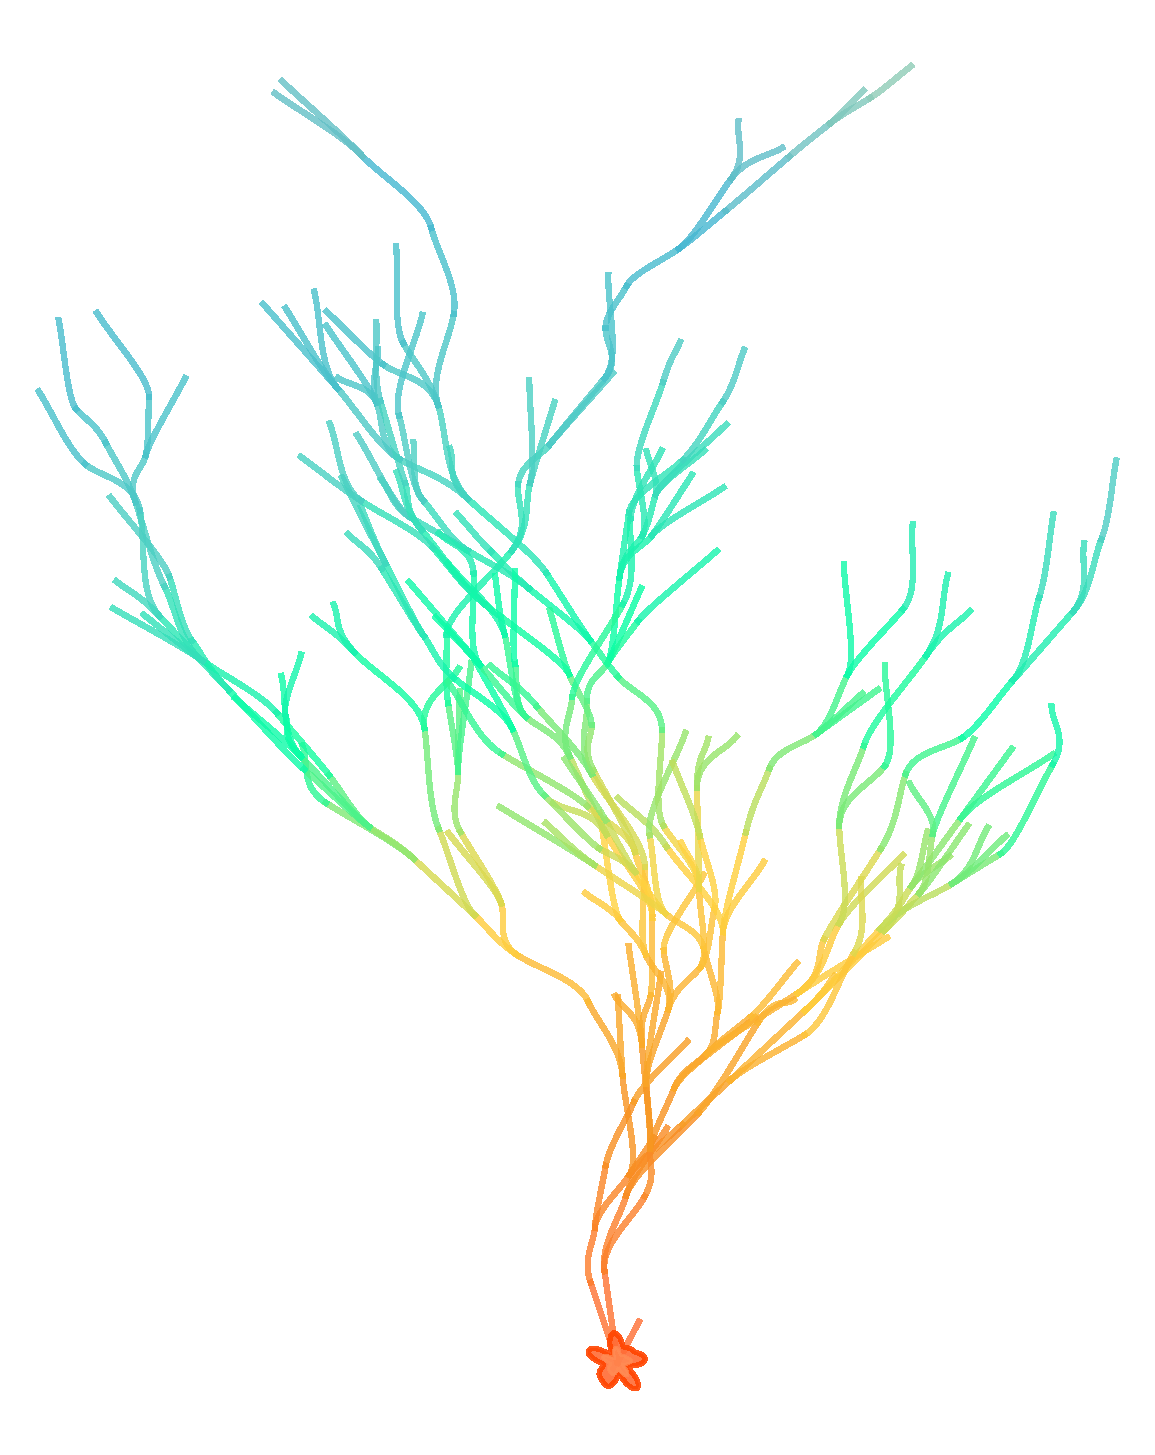
\includegraphics[width=0.25\textwidth]{assets/neuron_stylized.pdf}
        &
        {\Huge $\approx$}
        &
        \centering\begin{circuitikz}[scale=0.75, transform shape]
            % AC voltage source
            \draw (0,0) to[sV, v=$V_m(t)$] (0,3.5);
            \draw (0,3.5) to[short] (1.5,3.5);
            
            % Capacitor
            \draw (1.5,3.5) to[C, l=$C_m$] (1.5,0);
            
            % Connect to three branches
            \draw (1.5,3.5) to[short] (6.5,3.5);
            \draw (1.5,0) to[short] (6.5,0);
            
            % Sodium channel (Na+)
            \draw (3.2,3.5) to[vR, l=$g_{Na}$, *-] (3.2,2.0);
            \draw (3.2,2.0) to[battery1, l=$E_{Na}$] (3.2,0.5);
            \draw (3.2,0.5) to[short, -*] (3.2,0);
            
            % Potassium channel (K+)
            \draw (4.8,3.5) to[vR, l=$g_K$, *-] (4.8,2.0);
            \draw (4.8,2.0) to[battery1, l=$E_K$] (4.8,0.5);
            \draw (4.8,0.5) to[short, -*] (4.8,0);
            
            % Leak channel (Cl-)
            \draw (6.5,3.5) to[vR, l=$g_L$, *-] (6.5,2.0);
            \draw (6.5,2.0) to[battery1, l=$E_L$] (6.5,0.5);
            \draw (6.5,0.5) to[short, -*] (6.5,0);
            
            % Ground symbols
            \draw (0,0) node[ground]{};
            \draw (4.8,0) node[ground]{};
        \end{circuitikz}
    \end{tabular}
    \caption{Biological neuron and its Hodgkin-Huxley 
    equivalent circuit representation.}
    \label{fig:neuron_to_circuit}
\end{figure}

The corresponding differential equation describing the membrane potential dynamics is:
\begin{equation}
    C_m \frac{dV_m}{dt} = I_{ext} - g_{Na}(V_m - E_{Na}) - g_K(V_m - E_K) - g_L(V_m - E_L)
\end{equation}
where $I_{ext}$ is the external input current, and each conductance $g_i$ is voltage and time dependent, governed by additional gating variables.

However, as previously mentioned, natural system are often complex, as in this case we have a four dimensional non-linear coupled system, accurate modeling can be computationally infeasible, thus often simplified models are
preferred for large scale simulations, such as the Izhikevich neuron model \cite{1257420} that captures essential spiking dynamics with only two state variables.
\subsection{Discretization} \todo{quanto in dettaglio?}    

\clearpage

\section{Overview of Machine Learning}
Machine Learning (ML) is a subfield of Artificial Intelligence (AI) that focuses on statistical methods and algorithms capable to \textit{learn} from past experiences.
First we need a rigorous definition of what means to learn; \textcite[]{mitchell1997machine} defines it as : "A computer program is said to \textbf{learn} from experience $\mathbf{E}$ with respect to 
some class of tasks $\mathbf{T}$ and performance measure $\mathbf{P}$, if its performance at tasks in $\mathbf{T}$, as measured by $\mathbf{P}$, improves with experience $\mathbf{E}$."

ML can tackle a much wider range of tasks that are difficult to solve with explicit rules based programming, in a certain sense it bypasses
some level of abstraction, we're not learning the task $T$ directly, but we're sampling from the $E$ space, \textbf{examples} which are 
collection of \textbf{features} that are qualitative or quantitative properties of the data that are exploited by the model to learn the task $T$.%\newline
\subsection{The learning problem}
%Let's start with a definition
A formal definition of a machine learning model is given below:
\begin{comment}

\begin{definition}\todo{questo non è comunque abbastanza generico, perchè definisce solo supervised}
Given a I.I.D. unknown probability joint distribution $P(\mathbf{x}, y)$, with $D_{\text{train}} \sim P(\mathbf{x}, y)$, such that $\mathcal{D_{\text{train}}} = \{(\mathbf{x}_i, y_i)\}_{i=1}^{N} \in \mathcal{X} \times \mathcal{Y}$, where 
${\mathbf{x}_i} \in \mathbb{R}^d$ are the input features and ${y_i} \in \mathbb{R}$ (or $\{0,1\}$ for classification) are the target labels, then a \textbf{machine learning model} is a function $f:\mathbb{R}^d \rightarrow \mathbb{R}$ (or $\{0,1\}$) that maps $\mathbf{x}$ to $y$.
    The goal is to find the optimal parameters $\Theta^*$ of the model $f(\mathbf{x}; \Theta^*)$ that minimize a loss function $\mathcal{L}(y, f(\mathbf{x}; \Theta^*))$ over $\mathcal{D_{\text{train}}}$. 
    \footnote{This definition captures the \textit{supervised learning} paradigm. 
    More broadly, in \textit{unsupervised learning}, 
    the data consists only of $\{\mathbf{x}_i\}$ and 
    the goal is to learn the underlying structure of the data (e.g., clusters, latent representations,
     or the data distribution itself) by optimizing a task-specific objective function $\mathcal{J}$ 
     without the use of target labels $y$.}
\end{definition}

\end{comment}

\begin{definition}
Let $p_{\text{data}}(\mathbf{x})$ be an independent identically distributed (i.i.d.) unknown probability distribution over the input space $\mathcal{X}$. 
A dataset is a finite sample drawn from this distribution, $\mathcal{D} = \{\mathbf{x}_i\}_{i=1}^{N} \subset
 \mathcal{X}$, where $\mathbf{x}_i \in \mathbb{R}^d$ are data points (or input features).

A \textbf{machine learning model} is a family of prediction functions $f: \mathcal{X} \to \mathcal{Y}$ parameterized by 
$\theta$. The nature of the model and its goal is defined by the learning paradigm:

\begin{itemize}
    \item In the \textbf{supervised} setting, the data is drawn from a joint distribution $p_{\text{data}}(\mathbf{x}, y)$, 
    so $\mathcal{D}_{\text{train}} = \{(\mathbf{x}_i, y_i)\}_{i=1}^{N}$, with targets $y_i \in \mathcal{Y}$. 
    Here, $\mathcal{Y}$ (e.g., $\mathbb{R}$ for regression or $\{0,1\}$ for classification), 
    and the goal is to find parameters $theta^*$ that minimize a loss function $\mathcal{L}(y, f(\mathbf{x}; \theta))$ 
    quantifying the discrepancy between predictions and true labels.

    \item In the \textbf{unsupervised} setting, the data consists only of inputs $\mathbf{x}_i$. 
    The output space $\mathcal{Y}$ is defined by the specific task (e.g., $\mathbb{R}^k$ for dimensionality reduction, 
    a set of clusters for clustering, or $\mathbb{R}^d$ for generative models). The goal is to find parameters $\theta^*$
     that optimize an objective function $\mathcal{J}(f(\mathbf{x}; \theta), \mathcal{D})$,
      which captures desired structural properties of the data, such as reconstruction error, cluster cohesion, or data likelihood.
\end{itemize}

In both cases, the ultimate objective is for the model $f(\mathbf{x}; \theta^*)$ to generalize well to new, unseen data $\mathcal{D}_{\text{test}} \sim P(\mathbf{x})$. 
\end{definition}

The model $f_{\theta}$\footnote{We will use $f_{\theta}$ as shorthand for $f(\mathbf{x}; \theta)$}  is said to belong to a \textbf{hypothesis space} $\mathcal{H}$, 
which is the set of all possible functions the model can represent by varying its parameters $\theta$.
The choice of model architecture (e.g., linear models, neural networks, decision trees) 
defines the hypothesis space. A larger, more expressive $\mathcal{H}$ can represent more complex functions.
The learning algorithm searches within $\mathcal{H}$ to find the hypothesis 
$f^* = f(\cdot; \theta^*)$ that best approximates the true underlying relationship between inputs and outputs.
%\clearpage
\subsection{Learning Paradigms}
Models learn the data distributions in threen main different styles: \todo{c'è ne sono molti altri semisupervised, active learning etc.,}
\begin{enumerate}
    \item \textbf{Supervised Learning}, where the we aim for accurate predictions.
    \item \textbf{Unsupervised Learning}, tries to find a compact description of the data
    \item \textbf{Reinforcement Learning}, where an agent recursively interact with an environment in order to maximize a cumulative reward signal, trought a certain policy: $\pi^*$.
\end{enumerate} 
Understanding learning is crucial to choose the right modeling technique and architecture for a given task.
In order to have a more compact picture of learning let's decompose the more general distribution: $P(\mathbf{X}, Y)$

\begin{comment}
At the core of ML there are two main concepts: One we've seen before, the \textbf{Learning} process, 
which is the process of finding the optimal parameters $\Theta^*$ of the model such that the loss function $\mathcal{L}(y, f(\mathbf{x}; \Theta^*))$ is minimized with respect to training data, then we have \textbf{Generalization}, 
that is the capability to perform well on unseen data, given a certain distribution $P(\mathbf{x}, y)$. We can formalize these concept by examining how the joint distribution can be
decomposed and how this relates to the learning objective.\newline
\end{comment}
\subsubsection{Generative and Discriminative Learning o (bayesian view)}
The joint distribution $P(\mathbf{X}, Y)$ decomposes as: \todo{Vorrei evitare di spiegare bayes, ma come introduco questi concetti?}

\begin{equation}
    % color the marginal, prior, likelihood and posterior with different colors
    P(\mathbf{X}, Y) = \color{blue}{P(Y|\mathbf{X})}\color{red}{P(\mathbf{X})} 
    \color{black}= \color{green}{P(\mathbf{X}|Y)}\color{purple}{P(Y)}\color{black}
\end{equation}
\begin{equation*}
    \text{Joint} = \color{blue} \text{(Posterior)} \color{black} \cdot \color{red} \text{(Marginal)} \color{black} =
     \color{green} \text{(Likelihood)} \color{black} \cdot \color{purple} \text{(Prior)} \color{black}
\end{equation*}

In machine learning, the primary goal is often to predict the label $Y$ for a given datapoint
$\mathbf{X}$, this is represented by the \textit{posterior distribution}. One could also be interested in approximating the unknown distribution itself
to then generate new samples from it, in that case, are needed \textit{likelihood} and the \textit{prior} distributions.
\newline
% troppo didattico...
%By rewriting in terms of posterior distribution we get what is commonly referred as the \textbf{Bayes' Theorem}. \todo{citabayes}  
Bayesian Decision Theory \cite{barberBRML2011} provides a statistical framework for the design of many machine learning algorithms.
The way models parameters are estimated often reflects whether the approach is \textit{Generative} or \textit{Discriminative}.

\footnote{However, this correspondence is not absolute \cite[p.~312, Ch.~13]{barberBRML2011}: logistic regression
 can also be trained by pure MLE, and generative models can incorporate priors and thus be estimated via MAP.}
Discriminative models rely often on conditional distribution, the posterior, and whenever we can incorporate
prior knowledge on the parameters, inference is performed through \textbf{Maximum A Posteriori} (MAP) estimation \ref{eq:map}, which seek the best
hypotesis ($\theta$) given the data and prior knowledge.\newline


\todo{forse è meglio ridurre il numero di formule e tenerlo più discorsivo?}
\begin{equation}\label{eq:map}
\theta_{\text{MAP}}^* = \arg\max_{\theta} P(\theta|\mathcal{D}) = \arg\max_{\theta} P(\mathcal{D}|\theta)P(\theta)
\end{equation}

On the other hand generative models learn the joint distribution, and are typically trained by a \textbf{Maximum Likelihood Estimation} (MLE) \ref{eq:mle},
fitting the parameters that maximize the likelihood of the data.\newline
%questo era vecchio magari lo posso risusare se devo cambiare qualcosa
%%To do inference, we seek the best hypotesis a model can provide, which means finding the most probable parameters $\theta$ given the data, that's called Maximum A Posteriori (MAP) estimation:
\begin{equation}\label{eq:mle}
\theta_{\text{MLE}}^* = \arg\max_{\theta} P(\mathcal{D}|\theta)
|\theta)
\end{equation}

\subsection{Risk, Generalization and Overfitting o (Empirical view)}
%FOOTNOTE BARBER 13.3 CHAPTER PAGE 314
While the Bayesian perspective \footnote{As said in \cite[p.~314, Ch.~13]{barberBRML2011}, 
Bayesian approach appears to be formally optimal, but a pragmatic approach is possible, 
it can be conditioned by a penalty $\lambda$ on the complexity of the model} provides a probabilistic view for learning,
in practice what is often adopted is called the \textit{empirical} approach based on risk minimization
\cite{Vapnik1998}. This complements it by focusing on measuring and optimizing performance through the loss function,
with the main goal of achieving \textit{generalization}.
We seek a function $f_{\theta}$ that minimizes the expected risk $\mathcal{R}(f_\theta)$ over $p_{\text{data}}(\mathbf{x}, y)$.
The loss function acts as a proxy for the learning process, risk have a dual nature: the expected risk and the empirical risk.

The \textbf{expected risk} (or population risk) of a hypothesis $f_\theta$ measures its 
average performance over the true data distribution.
%
%\begin{equation}
%    \mathcal{R}(f_\theta) = \mathbb{E}_{(\mathbf{x}, y) \sim p_{\text{data}}}[\mathcal{L}(y, f(\mathbf{x}; \theta))]
%\end{equation}
However, we do not have access to the entire $p_{\text{data}}$ we can only observe a finite sample 
$\mathcal{D}_{\text{train}}$, therefore, we approximate 
the expected risk with the \textbf{empirical risk}: $\hat{\mathcal{R}}(f_\theta)$, which
is the average loss over the training set.\newline
%\begin{equation}
%    \hat{\mathcal{R}}(f_\theta) = \frac{1}{N}\sum_{i=1}^{N} \mathcal{L}(y_i, f(\mathbf{x}_i; \theta))
%\end{equation}
The learning problem becomes finding $\theta^*$ that minimizes $\hat{\mathcal{R}}(f_\theta)$ 
over the training set. This is the \textbf{Empirical Risk Minimization} (ERM) principle, 
which forms the foundation of most practical machine learning algorithms.
%The complete risk is thus divded into:
%\begin{equation}
    %% add also Optimization error
%   \mathcal{R}(f_\theta) = \underbrace{\hat{\mathcal{R}}(f_\theta)}_{\text{Empirical Risk}} + \underbrace{(\mathcal{R}(f_\theta) - \hat{\mathcal{R}}(f_\theta))}_{\text{Generalization Gap}}
%\end{equation}
%% Error is important we can decompose the expected error by Statistical Learning Theory

\subsubsection{Risk Decomposition}

%We choose $f_{\theta}$ from $\mathcal{H}$  such that the expected risk can be decomposed as:
Most of the times the space of possible solution is unfanthomably large, thus we need to decompose the risk in order to understand if 
we are generalizing correctly.\newline
Let $f_{\mathcal{H}}^* = \arg\min_{f \in \mathcal{H}} \mathcal{R}(f)$ be the best possible function within the hypothesis space, 
and let $\hat f_{\mathcal{H}} = \arg\min_{f \in \mathcal{H}} \hat{\mathcal{R}}(f)$ denote the empirical risk minimizer found by the learning algorithm.
Then, the population risk of the learned model can be decomposed in: \cite{10.5555/3360093}\cite{Vapnik1998}\cite{mjt_dlt}\cite[pag. 33, Ch 2]{bach2024learning}
%\cite{mjt_dlt}\cite[pag. 33 Ch 2]{bach2024learning}
%\cite[pag. 168, Ch 12.3]{books/daglib/0033642}

%The \textbf{approximation term} reflects the intrinsic limitations of the hypothesis space~$\mathcal{H}$, 
%the \textbf{generalization term} measures the difference between empirical and true performance, 
%and the \textbf{optimization term} accounts for the gap due to imperfect minimization of the empirical risk.

\begin{equation}
    \mathcal{R}(f_\theta) = 
    \underbrace{\mathcal{R}(f_\theta) - \hat{\mathcal{R}}(f_\theta)}_{\text{Generalization error}}
     + \underbrace{\hat{\mathcal{R}}(f_\theta) - \hat{\mathcal{R}}({f^*}_\mathcal{H})}_{\text{Optimization error}} 
     + \underbrace{\hat{\mathcal{R}}(\hat{f}_\mathcal{H}) - \mathcal{R}(f_\mathcal{H}^*)}_{\text{Estimation error}} + \underbrace{\mathcal{R}(f_\mathcal{H}^*)}_{\text{Approximation error}} 
\end{equation}

The approximation error is irreducible because the data-generating process includes 
an intrinsic noise~$\varepsilon$ that cannot be captured by any hypothesis
 in~$\mathcal{H}$. Consequently, learning algorithms must focus on reducing the remaining
  components. When the selected hypothesis~$f_\theta$ is insufficiently 
  expressive, \textbf{underfitting} occurs: the empirical risk $\hat{\mathcal{R}}(f_\theta)$ may be small,
   yet the estimated hypothesis fails to approximate the target function.\footnote{In the case of limited data availability}
    Conversely, if~$f_\theta$ possesses excessive capacity, the estimator
     can \textit{interpolate} $\mathcal{D}_{train}$, attaining negligible empirical risk, but with a large generalization gap; 
     this phenomenon is called \textbf{overfitting}. 

\subsection{Optimizing and Regularizing}\todo{questa è una parte più pragmatica che spiega come si fa learning e come si gestice la complessità}
We extensively talked about different ways of learning, but yet we haven't discussed on how actually the learning is performed.
Many of the modern ML algorithm are based on \textbf{Gradient-Based Optimization} methods \cite{citaqualcosa}, which iteratively update the model parameters $\theta$ in order to minimize the loss function $\mathcal{L}(y, f(\mathbf{x}; \theta))$.
% what we use for the learning in the work is mainly pseudoinverse, ridge regression since we rely on cover theorem
In this work we will focus on 
\todo{comunque nella tesi non facciamo molto uso di gradient based optimization, forse si può sorvolare sui dettagli o serve comunque come background?}
However learning differs from pure optimization, ML methods optimize indirectly with respect to the population risk.
% continua discorso su ottimizzazione e poi vai direrramente sulla parte successiva
The typical ML objective function minimized is:
\begin{equation}
    \mathcal{L(\theta)} = \mathbb{E}_{(\mathbf{x}, y) \sim \mathcal{D}_{train}}[\mathcal{L}(y, f(\mathbf{x}; \theta))] + \lambda \Omega(\mathbf{w}) 
\end{equation}

The term $\Omega(\mathbf{w})$ is a regularization term that allows to control the complexity of the model, $\lambda$
is an hyperparameter that controls the strength of the regularization.

The most common algorithm is the \textbf{Stochastic Gradient Descent} (SGD) \cite{citaqualcosa}, 
which iteratively updates the parameters $\theta$ in the opposite direction of the gradient of the loss function with respect to the parameters.
Typically we start from a configuration $\theta_0$ and at each iteration $t$ we compute the gradient of the loss function
with respect to the parameters $\nabla_\theta \mathcal{L}(\theta_t)$, then we update the parameters using a learning rate $\eta$ that controls the step size of the update.

The learning rule is written as:

\begin{equation}
    \theta_{t+1} = \theta_t - \eta \nabla_\theta \mathcal{L}(\theta_t)
\end{equation}

\subsubsection{Optimization and Regularization in Reservoir Computing} \todo{questa parte va spostata, metterla qui è troppo presto, oppure introduco reservoir prima}
In reservoir computing, the recurrent connections remains fixed after initialization, 
so learning reduces to estimating the readout parameters. 
Given reservoir states collected in the recurent matrix $\mathbf{W_{rec}} \in \mathbb{R}^{N \times d}$
 and targets $\mathbf{Y} \in \mathbb{R}^{N \times m}$, the readout weights $\mathbf{W_{out}} \in \mathbb{R}^{d \times m}$ are obtained by solving a regularized least-squares problem:

\begin{equation}
    \mathbf{W_{out}} = \arg\min_{\mathbf{W}} ||\mathbf{Y} - \mathbf{W}^T \mathbf{W_{rec}}||_2^2 + \lambda ||\mathbf{W}||_2^2
\end{equation}

The Tikhonov coefficient $\lambda \ge 0$ controls the readout capacity and mitigates overfitting. whenever
$N$ or $d$ is large, iterative solvers such as conjugate gradients approximate the same optimum while retaining the regularization term.

\subsubsection{Model selection and Hyperparameters}

\section{Structured Probabilistic Models (Graphical Models)}\todo{Since RNN are Directed Graphical Models}
Qui l'idea è di andare a parlare dei modelli grafici probabilistici e di come questi siano utili per capire i modelli neurali su sequenze

Structured Probabilistic Models are used to describe a probability distribution using a graph (from graph theory) structure,
which nodes represent random variables and edges represent dependencies between them.

What need to add: Directed and Undirected, inference and learning basics, few famous models (HMM, RBM, CRF Energy-Based Models (EBM),
 why structured models are so useful : Information flow, interpretability, prior knowledge, etc.)

\begin{comment}
% filepath: /home/vincent/UniversityNotes/Thesis/notes/chapters/background.tex
\begin{figure}[H]
    \centering
    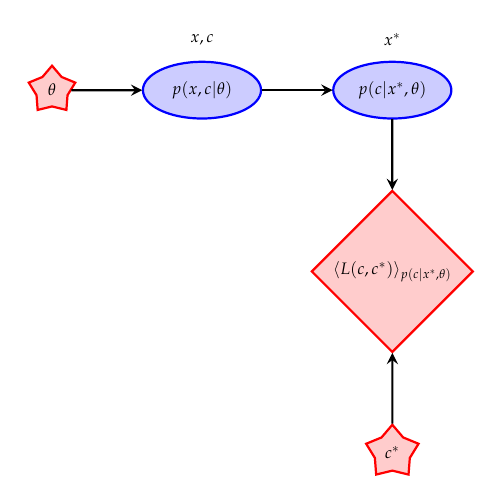
\begin{tikzpicture}[
        node distance=1.5cm,
        thick,
        >=stealth,
        scale=0.6,
        transform shape
    ]
    
    % Nodes with simple styles
    \node[star, star points=5, minimum size=8mm, draw=red, fill=red!20] (theta) {$\theta$};
    \node[ellipse, minimum width=25mm, minimum height=12mm, draw=blue, fill=blue!20, right=of theta] (p1) {$p(x,c|\theta)$};
    \node[ellipse, minimum width=25mm, minimum height=12mm, draw=blue, fill=blue!20, right=of p1] (p2) {$p(c|x^*,\theta)$};
    \node[diamond, minimum width=30mm, minimum height=15mm, draw=red, fill=red!20, below=of p2] (loss) {$\langle L(c,c^*)\rangle_{p(c|x^*,\theta)}$};
    \node[star, star points=5, minimum size=8mm, draw=red, fill=red!20, below=of loss] (cstar) {$c^*$};
    
    % Input/output labels
    \node[above=2mm of p1] {$x,c$};
    \node[above=2mm of p2] {$x^*$};
    
    % Simple arrows
    \draw[->] (theta) -- (p1);
    \draw[->] (p1) -- (p2);
    \draw[->] (p2) -- (loss);
    \draw[->] (cstar) -- (loss);
    
    \end{tikzpicture}
    \caption{Probabilistic graphical model representation}
    \label{fig:probabilistic_model}
\end{figure}
\end{comment}


\section{Recurrent Neural Networks and Deep Learning}
yadaydayda

\section{Deep Recurrent Neural Networks}\todo{questa parte va riscritta dopo}
Deep Learning had a great impact on the field of machine learning and artificial intelligence. When we consider a 
deep learning model, we are referring to a model that has multiple layers of neurons. 
The most common type of deep learning model is the Multilayer Perceptron (MLP),
 which consists of multiple layers of fully connected neurons. By adding layers to these models
 we are able to learn representation at different scales, each layer take the pattern from the previous layers and is capable 
 to learn a more complex pattern. 
 In this work, we will focus on
 a set of deep learning models known as Recurrent Neural Networks (RNNs).\cite{ELMAN1990179}\todo[color=green!90]{citations needed}
 RNNs are a type of neural network that is designed to handle sequential data. Depth in these architectures usually referes
 to the number of timestep we unroll the network trough time (or sequence). But we can add depth in more than one way,
 one of those is to stack multiple layers of RNNs on top of each other sequentially. 
 
 \todo{Change this image or make a new one or cite it}
 \begin{figure}[H]
    \centering
    \includegraphics[width=0.9\textwidth]{images/deep_architectures.png}
    \caption{Depths in Neural Network}
    \label{fig:rnn}
\end{figure}

\section{Deep Reservoir Computing}\todo{questo vai nei related works}

Reservoir Computing (RC) is a framework introduced by \todo[color=green!90]{cite}, that is designed to 
simplify the training of Recurrent Neural Networks. 
The main point is that we do not need to train the recurrent connections
 of the network, but only an output layer called the readout.

\chapter{Methodology}\label{ch:methodology}
% --- Core Variables (with arguments for layer index) ---
% Usage: \hState{l} -> h^(l)_t
\newcommand{\hState}[1]{\mathbf{h}^{(#1)}_t}

% Usage: \Win{l} -> W_in^(l)
\newcommand{\Win}[1]{\mathbf{W}_{\text{in}}^{(#1)}}

% Usage: \Wrec{l} -> W_rec^(l)
\newcommand{\Wrec}[1]{\mathbf{W}_{\text{rec}}^{(#1)}}

% Usage: \Wcyc{l} -> W_cyc^(l)
\newcommand{\Wcyc}[1]{\mathbf{W}_{\text{cyc}}^{(#1)}}


% Usage: \bias{l} -> b^(l)
\newcommand{\bias}[1]{\mathbf{b}^{(#1)}}

% --- Coupling Matrices ---
% Usage: \Cfwd{l} -> C^(l)_forward
\newcommand{\Cfwd}[1]{\mathbf{C}^{(#1)}_{\rightarrow}}
\newcommand{\Cbwd}[1]{\mathbf{C}^{(#1)}_{\leftarrow}}

% --- Total Weight Matrices ---
% Note: Using 'bmatrix' (bracketed matrix) is standard for linear algebra. 
% If you strictly want no brackets, change back to 'matrix'.

\newcommand{\WDeepESN}{
    \begin{bmatrix}
    \Wrec{1} & \mathbf{0} & \cdots & \mathbf{0} \\
    \Win{2} & \Wrec{2} & \cdots & \mathbf{0} \\
    \vdots & \ddots & \ddots & \vdots \\
    \mathbf{0} & \cdots & \Win{L} & \Wrec{L}
    \end{bmatrix}
}

\newcommand{\WtotCycle}{
    \begin{bmatrix}
    \Wrec{1} & \mathbf{0} & \cdots & \mathbf{\Wcyc{1}} \\
    \Wcyc{2} & \Wrec{2} & \cdots & \mathbf{0} \\
    \vdots & \ddots & \ddots & \vdots \\
    \mathbf{0} & \cdots & \Wcyc{L} & \Wrec{L}
    \end{bmatrix}
}

\newcommand{\WtotAntisym}{
    \mathbf{W}_{\text{diag}} +
    \epsilon
    \begin{bmatrix}
    \mathbf{0} & -\Cbwd{1}^\top & \cdots & \mathbf{0} \\
    \Cfwd{1} & \mathbf{0} & \ddots & \vdots \\
    \vdots & \ddots & \ddots & -\Cbwd{L-1}^\top \\
    \mathbf{0} & \cdots & \Cfwd{L-1} & \mathbf{0}
    \end{bmatrix}
}

% !TeX root = ../../main.tex
\label{chap:methodology}
After having discussed all the background concepts and related works, we can now move on to the methodology used in this work
In this chapter we present the idea to treat deep recurrent neural network as \emph{modular deep reservoir} architectures. 
%We will discuss about modularity in RNNs and the two proposed architectures in details. 
Rather than treating reservoir as a monolithic recurrent system, we interpret each layer of the deep reservoir as an independent computational module that processes inputs and exchanges information with other modules through structured interconnections.
The central objective is to study how architectural constraints \ref{...} antisymmetric dynamics with \emph{forward and backward} inter-module coupling, and \ref{...} a \emph{cycle-based} affect stability, memory retention and performance on sequence learning tasks.
\todo{finire di scrivere questo quando avrò un idea di come sara fatta la metodologia}

\section{Modularity in RNNs}
\label{sec:method:modularity}
In dynamical systems theory, a system is said to be \emph{modular} if it can be decomposed into distinct 
subsystems (modules) each of which has its own internal dynamics while also interactting with other modules.
Such composition allows for a complex global behaviour to emerge from the interactions of simpler components.
At the same time, analyzing the system in terms of local module dynamics can provide control on information flow and interpretability benefits.

Modularity has been extensively studied in neuroscience, where large-scale brain networks exhibit modular organization with specialized regions that acts as hubs for information integration.
Empirical studies from Bullmore et al. \cite{bullmore2009complex} have shown that neural systems are composed of densely connected subnetworks that interact globally as a sparse system \todo{che sono connesse in modo sparso forse è meglio?}, supporting
both integration of information and specialized processing 

More generally, studies in complex systems and network dynamics have shown that modular organization 
can enhance robustness by inducing a separation of time scales, such that dynamical processes remain
 confined within subsystems for extended periods before spreading globally. 
 This structure allows perturbations to decay locally and supports stable large-scale 
 dynamics under appropriate stability conditions \cite{Lambiotte_Schaub_2022}.

In this work, we take inspiration from these principles to design deep reservoir architectures, which hierachical structure
can be further enriched with modular interconnections promoting richer dynamics and preserving stability and memory.

\todo{Forse quando parlo in questo modo della modularità nella tesi dovrei anche dire che stiamo trattando le architetture deep "normali" come se fossero    moduli o è già sottinteso?}

\begin{comment}
We consider supervised learning on temporal data.
Given an input sequence $\{\mathbf{u}(t)\}_{t=1}^{T}$ with $\mathbf{u}(t)\in\mathbb{R}^{d_u}$, a reservoir system produces a sequence of hidden states $\{\mathbf{x}(t)\}_{t=1}^{T}$, $\mathbf{x}(t)\in\mathbb{R}^{d_x}$, from which an output sequence $\{\mathbf{y}(t)\}_{t=1}^{T}$ is predicted:
\begin{equation}
    \hat{\mathbf{y}}(t) = \mathbf{W}_{\text{out}} \, \boldsymbol{\phi}(\mathbf{z}(t)) + \mathbf{b}_{\text{out}},
    \label{eq:method:readout}
\end{equation}
where $\mathbf{z}(t)$ is a concatenation of features (e.g., reservoir states across modules and optionally the input), and $\boldsymbol{\phi}(\cdot)$ is a (possibly identity) feature map.
In standard reservoir computing (RC), only the readout parameters $(\mathbf{W}_{\text{out}}, \mathbf{b}_{\text{out}})$ are trained.
\end{comment}
%\clearpage
\section{Deep Modular Reservoirs}
\label{sec:method:deep_modular}
We model a deep reservoir as a composition of $L$ layers or modules. 
Each module $l\in\{1,\dots,L\}$ has state $\mathbf{h}^{(l)}(t)\in\mathbb{R}^{n_l}$ and internal recurrent connectivity $\mathbf{W}^{(l)}$.
The key methodological contribution is to compare two architectures of deep modular reservoirs:

\begin{itemize}
    \item \textbf{Antisymmetric deep reservoir} with \emph{forward and backward} coupling between adjacent modules, designed to promote stable dynamics and improve gradient-free memory propagation.
    \item \textbf{Cycle deep reservoir} where we emply \emph{cycle/ring} recurrent topology, inspired by Simple Cycle Reservoirs (SCR), to provide strong memory traces with minimal parameters.
\end{itemize}

\subsection{Global state and dynamics}
Let $\mathbf{y}(t)$ be the global reservoir state at time $t$ obtained by feeding the input $\mathbf{u}(t)$ into the first module and propagating through the layers.
By stacking the states of all modules, we have the final feature vector used for the readout is made
\begin{equation}
    \mathbf{y}(t) = \begin{bmatrix}
    \mathbf{h}^{(1)}(t) \\
    \mathbf{h}^{(2)}(t) \\
    \vdots \\
    \mathbf{h}^{(L)}(t)
    \end{bmatrix} \in \mathbb{R}^{N}, \quad N = \sum_{l=1}^L n_l.
    \label{eq:method:feature_concat}
\end{equation}
Where $N$ is the total reservoir size and $n_l$ is the size of module $l$.
The global dynamics of the reservoir can be written in the compact form:
obtained after the application of the activation function and leaky integration.

We define the pre-activation vector
\begin{equation}
\mathbf z(t+1) =
\mathbf W_{\text{tot}} \mathbf y(t)
+ \mathbf W_{\text{in}} \mathbf x(t+1)
+ \mathbf b .
\end{equation}

The reservoir state is then updated as
\begin{equation}
\mathbf y(t+1) =
(1-\alpha)\mathbf y(t) + \alpha f(\mathbf z(t+1)).
\end{equation}
\begin{equation}
\mathbf{y}(t+1) = f\left(\mathbf{W}_{\text{tot}} \, \mathbf{y}(t)\right),
\end{equation}
where $f(\cdot)$ acts element-wise on the state vector and
$\mathbf{W}_{\text{tot}} \in \mathbb{R}^{N \times N}$ encodes both intra-module and inter-module connections.


where $\mathbf{W}_{\text{tot}} \in \mathbb{R}^{N \times N}$ is a block matrix that encodes both intra-module and inter-module connections.
For a simple Leaky-ESN with 1 layer, the $\mathbf{W}_{\text{tot}}$ is simply the recurrent weight matrix $\mathbf{W}_{\text{rec}}$ of the reservoir.

So the structure of $\mathbf{W}_{\text{tot}}$ depends on the chosen architecture, a randomly connected module architecture would have 
a block diagonal structure, plus random connections between modules.

\subsubsection{DeepESN as modular system}
In the paper from \cite{GALLICCHIO201787} the authors propose to study what happens when treating modules as a stack, 
hence, in DeepESN architecture with $L$ layers where information is processed hierachically have a matrix for the entire system $W_{\text{DeepESN}}$ in the following form: 

\begin{equation}
    W_{\text{DeepESN}} =\WDeepESN
\end{equation}

Where each block on the diagonal represents the recurrent connections of each module, and the sub-diagonal blocks represent the input connections from the previous layer.
When a single input perturbation is applied, deeper layers retain the perturbation for longer,
 indicating that higher layers capture slower (low‑frequency) temporal components and lower layers capture faster (high‑frequency) components, this is likely due to the fading
 memory effect of the reservoir dynamics.
This indicates that increasing the distance between the input and subsequent layers is crucial for developing a rich spectrum of temporal dynamics
The mechanism of capturing different components of frequency spectrum of the signal is very similar to the one observed in Convolutional Neural Networks (CNNs) for image processing, 
where lower layers capture high-frequency details and higher layers capture low-frequency structures.\todo{forse questo è inutile da dire}

% insert image of deep esn svg
\begin{figure}[ht!]
    \centering
    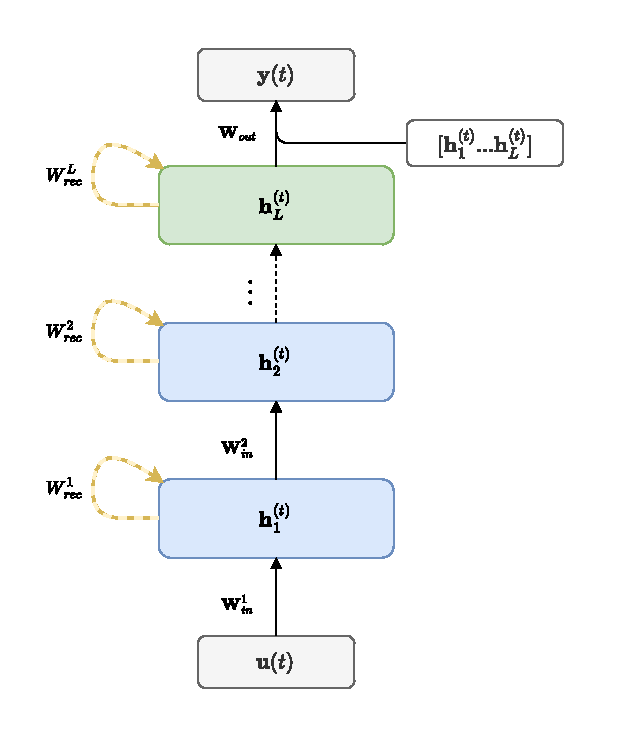
\includegraphics[width=0.5\textwidth]{images/modular_deepesn.pdf}
    \caption{Modular structure of a standard DeepESN. Each layer acts as an independent module with feedforward inter-layer communication.}
\end{figure}

%%%%%%%%%%%%%%%%%%%%%%%%%%%%%%%
\clearpage
\section{Deep Cycle Reservoir}
\label{sec:method:cycle}
The first architecture we propose is inspired to the work of Rodan and Tino \cite{mincomplex}, discussed in sec. \ref{sec:method:cycle}, they
introducing simple and deterministic reservoir models, such as the Simple Cycle Reservoir (SCR), which use a fixed ring topology for the recurrent connections.

\subsection{Motivation}
In a conventional deep ESN, information flows unidirectionally 
from the input through the stacked reservoirs to the readout.
But it lacks a feedback path that might allow higher‑level temporal abstractions
  to influence lower levels. A cyclic deep reservoir introduces a feedback connection 
  from the output of the last reservoir layer back to the first layer.
   The motivation for closing the loop is to allow information processed at deeper layers 
   (capturing longer‑term or low‑frequency features) to inform the processing of new inputs.
    This can enrich the reservoir dynamics and, in principle, improve tasks requiring both short and long‑term memory.


\subsection{Deep Cycle}
We can define the equation for the Deep Cycle Reservoir as follows:

\begin{equation}
    \label{eq:method:cycle_dynamics}
    \begin{cases}
    \mathbf{h}^1{(t)} = (1 - \alpha) \mathbf{h}^1{(t-1)} + \alpha \tanh\left(W_{\text{in}}^{(1)} \mathbf{u{(t)}} + W_{\text{rec}}^{(1)} \mathbf{h}^1{(t-1)} + \math{W}_{cyc}^1 \mathbf{h}^{L}{(t-1)}\right) \\  \\
    \mathbf{h}^l{(t)} = (1 - \alpha) \mathbf{h}^l{(t-1)} + \alpha \tanh\left(W_{\text{in}}^{(l)} \mathbf{u{(t)}} + W_{\text{rec}}^{(l)} \mathbf{h}^l{(t-1)} + \math{W}_{cyc}^l \mathbf{h}^{l-1}{(t-1)}\right) 
    \end{cases}
\end{equation}

We have a (cycle) matrix $W_{cycle}$ with:

\begin{equation}
    W_{cycle}=a\WtotCycle
\end{equation}

Where each $\Wrec{l}$ is scaled by $\rho$ and $\Wcyc{l}$ is initialized as same as recurrent matrices but can have different $\rho$ scaling factor.
The $\rho$ controls the effective spectral radius (for a pure permutation cycle, the eigenvalues lie on the unit circle, and scaling by $\rho$ sets their magnitude).

\subsection{Deep coupling for cycle modules}
We use a forward coupling between modules (and optionally bidirectional coupling as an ablation):
\begin{align}
    \tilde{\mathbf{x}}^{(\ell)}(t+1)
    &= \tanh\!\Big(
        \mathbf{W}^{(\ell)} \mathbf{x}^{(\ell)}(t)
        + \mathbf{W}^{(\ell)}_{\text{in}} \mathbf{h}^{(\ell)}(t+1)
        + \mathbf{C}^{(\ell)} \mathbf{x}^{(\ell-1)}(t)
        + \mathbf{b}^{(\ell)}
    \Big),\\
    \mathbf{x}^{(\ell)}(t+1)
    &= (1-\alpha_\ell)\mathbf{x}^{(\ell)}(t) + \alpha_\ell \tilde{\mathbf{x}}^{(\ell)}(t+1).
\end{align}
This creates a \emph{cycle-based deep reservoir} where each layer has a controlled internal topology and the depth contributes compositional temporal features.


% proof of bounding eigenvlaues
\begin{proof}
    \section{Stability Analysis of Deep Cycle Reservoir via Gershgorin Circle Theorem}

To guarantee the Echo State Property (ESP) and asymptotic stability of the Deep Cycle Reservoir, we analyze the spectral radius of the system's Jacobian. We consider a deep architecture with $L$ layers, where the state update for the $l$-th layer is given by:

\begin{equation}
    \mathbf{h}^{(t)}_l = (1-\alpha)\mathbf{h}^{(t-1)}_l + \alpha \tanh\left( \mathbf{W}_{in}^{(l)}\mathbf{u}^{(t)} + \mathbf{W}_{rec}^{(l)}\mathbf{h}^{(t-1)}_l + \mathbf{W}_{proj}^{prev}\mathbf{h}^{(t-1)}_{prev} \right)
\end{equation}

where $\mathbf{h}_{prev}$ denotes $\mathbf{h}_{l-1}$ for $l > 1$, and $\mathbf{h}_{L}$ for the first layer $l=1$ (closing the cycle).

\subsection{Jacobian Construction}
The effective global weight matrix $\mathbf{J}$ governing the linearized dynamics of the coupled system is a block-circulant-like matrix:

\begin{equation}
    \mathbf{J} = \bigoplus_{l=1}^L \left[ (1-\alpha)\mathbf{I} + \alpha \mathbf{W}_{rec}^{(l)} \right] + \alpha \mathbf{W}_{cycle}
\end{equation}

where $\mathbf{W}_{cycle}$ contains the inter-layer projection blocks $\mathcal{W}_{proj}$ on the sub-diagonal (and top-right).

\subsection{Gershgorin Bound Derivation}
According to the Gershgorin Circle Theorem, the spectrum of $\mathbf{J}$, $\sigma(\mathbf{J})$, is contained within the union of discs $D_i(c_i, R_i)$, where $c_i$ is the diagonal entry and $R_i$ is the sum of the absolute values of the off-diagonal entries of the $i$-th row.

For a neuron $k$ in layer $l$, the center $c_{l,k}$ and radius $R_{l,k}$ are derived as follows:

\begin{enumerate}
    \item \textbf{Center ($c_{l,k}$):} 
    Assuming the recurrent weight matrix $\mathbf{W}_{rec}^{(l)}$ has a zero main diagonal (as in the Simple Cycle Reservoir topology), the diagonal comes solely from the leakage term:
    \begin{equation}
        c_{l,k} = 1 - \alpha
    \end{equation}
    
    \item \textbf{Radius ($R_{l,k}$):}
    The radius is the sum of the magnitudes of incoming weights from two sources: the recurrent connections within layer $l$ and the projection connections from the previous layer in the cycle.
    \begin{equation}
        R_{l,k} = \alpha \left( \sum_{j} |(\mathbf{W}_{rec}^{(l)})_{kj}| + \sum_{p} |(\mathcal{W}_{proj})_{kp}| \right)
    \end{equation}
\end{enumerate}

\subsection{Initialization Specifics}
We evaluate the bound based on the specific initialization schemes used in this work:

\textbf{Case 1: Simple Cycle Reservoir (SCR) Topology} \\
Using the initialization from \texttt{scr.py}, the recurrent matrix $\mathbf{W}_{rec}$ forms a ring where each row has exactly one non-zero element with magnitude $r$. The projection matrix $\mathcal{W}_{proj}$ is initialized (via \texttt{utils.py}) such that the maximum absolute row sum is bounded by a projection strength $\gamma$.
\begin{align}
    \sum_{j} |(\mathbf{W}_{rec}^{(l)})_{kj}| &= r \\
    \sum_{p} |(\mathcal{W}_{proj})_{kp}| &\le \gamma
\end{align}
Substituting these into the Gershgorin radius:
\begin{equation}
    R_{l,k} = \alpha (r + \gamma)
\end{equation}

\textbf{Stability Condition} \\
For stability, we require the spectral radius $\rho(\mathbf{J}) < 1$. By the theorem, it suffices that the largest Gershgorin disc lies entirely within the unit circle. Since the center is at $1-\alpha$ (on the positive real axis), the condition becomes:
\begin{equation}
    c_{l,k} + R_{l,k} < 1 \implies (1 - \alpha) + \alpha(r + \gamma) < 1
\end{equation}

Simplifying the inequality, we obtain the sufficient condition for the Deep Cycle Reservoir:
\begin{equation}
    \boxed{r + \gamma < 1}
\end{equation}

This result proves that in a Deep Cycle architecture initialized with SCR blocks, the sum of the recurrent weight $r$ and the effective projection strength $\gamma$ must be strictly less than 1 to theoretically guarantee the Echo State Property via Gershgorin analysis.
\end{proof}


\section{Deep Antisymmetric Reservoir}
\label{sec:method:antisymmetric}

\subsection{Motivation}
Antisymmetric (or skew-symmetric) connectivity can constrain the dynamics in a way that mitigates exploding trajectories.
Intuitively, purely antisymmetric linear dynamics preserve energy in continuous time; in practice, discrete-time nonlinear systems may still benefit from the improved conditioning and stability induced by such constraints.

\subsection{Module dynamics}
For module $\ell$, we use a leaky update of the form:
\begin{align}
    \tilde{\mathbf{x}}^{(\ell)}(t+1)
    &= \tanh\!\Big(
        \mathbf{W}^{(\ell)} \mathbf{x}^{(\ell)}(t)
        + \mathbf{W}^{(\ell)}_{\text{in}} \mathbf{h}^{(\ell)}(t+1)
        + \mathbf{C}^{(\ell)}_{\rightarrow}\mathbf{x}^{(\ell-1)}(t)
        + \mathbf{C}^{(\ell)}_{\leftarrow}\mathbf{x}^{(\ell+1)}(t)
        + \mathbf{b}^{(\ell)}
    \Big), \label{eq:method:antisym_pre}\\
    \mathbf{x}^{(\ell)}(t+1)
    &= (1-\alpha_\ell)\mathbf{x}^{(\ell)}(t) + \alpha_\ell \tilde{\mathbf{x}}^{(\ell)}(t+1),
    \label{eq:method:antisym_leak}
\end{align}
where $\alpha_\ell\in(0,1]$ is a leak rate.
We set $\mathbf{x}^{(0)}(t)\equiv \mathbf{0}$ and $\mathbf{x}^{(L+1)}(t)\equiv \mathbf{0}$ (or omit missing terms at the boundaries).
The signal $\mathbf{h}^{(\ell)}(t+1)$ is the input to module $\ell$:
\begin{equation}
    \mathbf{h}^{(1)}(t+1) = \mathbf{u}(t+1), \qquad
    \mathbf{h}^{(\ell)}(t+1) = \mathbf{x}^{(\ell-1)}(t) \ \text{for}\ \ell\ge 2
\end{equation}
(or an alternative design depending on the experiment; this is explicitly controlled in ablations).

\subsection{Antisymmetric parametrization}
To construct an antisymmetric recurrent matrix, we sample a raw matrix $\mathbf{A}^{(\ell)}$ and set:
\begin{equation}
    \mathbf{W}^{(\ell)} = \gamma_\ell \left(\mathbf{A}^{(\ell)} - \mathbf{A}^{(\ell)\top}\right),
    \label{eq:method:antisym_W}
\end{equation}
where $\gamma_\ell>0$ controls the effective scale (optionally followed by spectral normalization).
Coupling matrices $\mathbf{C}^{(\ell)}_{\rightarrow}$ (forward) and $\mathbf{C}^{(\ell)}_{\leftarrow}$ (backward) are initialized as sparse random matrices and rescaled by coupling strengths $c_{\rightarrow}$ and $c_{\leftarrow}$.
This yields a \emph{bidirectionally coupled} deep reservoir, enabling information flow from lower to higher modules and feedback from higher to lower modules.

\subsection{Coupling ablations}
To isolate the effect of bidirectionality, we evaluate:
\begin{itemize}
    \item \textbf{Forward-only}: $\mathbf{C}^{(\ell)}_{\leftarrow}=\mathbf{0}$.
    \item \textbf{Backward-only}: $\mathbf{C}^{(\ell)}_{\rightarrow}=\mathbf{0}$.
    \item \textbf{Bidirectional}: both terms active.
\end{itemize}

\section{Initialization and Hyperparameters}
\label{sec:method:hyperparams}

Across both architectures, we control:
\begin{itemize}
    \item \textbf{Module sizes} $\{n_\ell\}_{\ell=1}^L$ and depth $L$.
    \item \textbf{Leak rates} $\alpha_\ell$ (shared or per-layer).
    \item \textbf{Input scaling} for $\mathbf{W}^{(\ell)}_{\text{in}}$ and coupling scaling for $\mathbf{C}$ matrices.
    \item \textbf{Spectral scaling}: $\gamma_\ell$ for antisymmetric modules or $\rho_\ell$ for cycle modules.
    \item \textbf{Readout regularization} $\lambda$ in Eq.~\eqref{eq:method:ridge}.
\end{itemize}

All random matrices are initialized from zero-mean distributions (Gaussian or uniform) and then rescaled to match target norms/sparsity.
We repeat experiments across multiple random seeds to estimate variance.

\section{Training and Evaluation Protocol}
\label{sec:method:protocol}

\subsection{Data preprocessing}
Inputs are standardized per feature (mean $0$, variance $1$) when applicable.
For classification tasks, targets are one-hot encoded; for regression, targets are optionally standardized and rescaled back for reporting.

\subsection{Washout}
To reduce dependence on the initial state, we discard an initial \emph{washout} segment of length $T_{\text{w}}$.
Only states $\{\mathbf{z}(t)\}_{t=T_{\text{w}}+1}^{T}$ are used for training and evaluation.

\subsection{Metrics}
We report:
\begin{itemize}
    \item \textbf{Classification}: accuracy (and macro-F1 when class imbalance is present).
    \item \textbf{Regression}: mean squared error (MSE) and normalized RMSE (when appropriate).
    \item \textbf{Memory}: memory capacity (MC) or task-specific memory measures when included in the benchmark suite.
\end{itemize}

\subsection{Baselines}
We compare the proposed architectures against:
\begin{itemize}
    \item A standard single-layer ESN with comparable total state dimension.
    \item A deep ESN with forward-only coupling (when the proposed model is bidirectional).
    \item A structured SCR-like single module (when evaluating the benefit of depth).
\end{itemize}

\section{Ablation Studies}
\label{sec:method:ablations}

We perform controlled ablations to attribute performance gains:
\begin{enumerate}
    \item \textbf{Coupling directionality}: forward vs backward vs bidirectional.
    \item \textbf{Structure vs randomness}: antisymmetric/cycle $\mathbf{W}^{(\ell)}$ vs dense random $\mathbf{W}^{(\ell)}$ under matched scaling.
    \item \textbf{Depth vs width}: varying $L$ while keeping total state size $\sum_\ell n_\ell$ fixed.
    \item \textbf{Readout features}: last-layer-only vs concatenation across layers (Eq.~\eqref{eq:method:feature_concat}).
\end{enumerate}

\section{Implementation Notes}
\label{sec:method:implementation}

All models are implemented in Python with vectorized state updates.
For reproducibility, experiments log the random seed, hyperparameters, and the exact dataset split.
Unless otherwise specified, only the linear readout is trained, enabling efficient training via closed-form ridge regression (Eq.~\eqref{eq:method:ridge}).

\section{Summary}
\label{sec:method:summary}

The methodology evaluates two modular deep reservoir families:
(1) antisymmetric modules with bidirectional coupling to study stability and information flow,
and (2) cycle-based (SCR-like) modules to study the effect of strong structural priors.
Both are trained with identical readout procedures and compared under matched experimental controls to isolate architectural effects.

\subsection{Modular Interpretation of Deep Reservoir Architectures}

All architectures considered in this work can be interpreted as \emph{modular dynamical systems}, where each reservoir layer acts as an autonomous computational module.
Each module consists of a fixed number of recurrent units that process incoming signals and exchange information with other modules according to a prescribed connectivity pattern.

Let each module $l \in \{1,\dots,L\}$ be associated with a state vector
$\mathbf{h}^{(l)}_t \in \mathbb{R}^{N_l}$, where $N_l$ is the number of units in the layer.
Modules interact exclusively through linear projections of their internal states, while nonlinear processing occurs locally within each module.

This modular view allows the architecture to be analyzed in terms of structured interconnections between subsystems, rather than as a monolithic recurrent network.

\subsection{Standard DeepESN: Hierarchical Modularity}

In a standard DeepESN without cyclic or antisymmetric connections, information flows strictly forward across layers.
The global recurrent matrix has a \emph{block lower-triangular} structure:
\begin{equation}
\mathbf{W}_{\text{tot}} =
\begin{bmatrix}
\mathbf{W}_{rec}^{(1)} & \mathbf{0} & \cdots & \mathbf{0} \\
\mathbf{W}_{in}^{(2)} & \mathbf{W}_{rec}^{(2)} & \cdots & \mathbf{0} \\
\vdots & \ddots & \ddots & \vdots \\
\mathbf{0} & \cdots & \mathbf{W}_{in}^{(L)} & \mathbf{W}_{rec}^{(L)}
\end{bmatrix}.
\end{equation}

Each diagonal block represents the internal dynamics of a module, while sub-diagonal blocks model feedforward communication between adjacent modules.
This structure implies that the Jacobian of the system is block lower-triangular, and its spectral radius is governed by the most unstable module.

\begin{figure}[t]
    \centering
    % TODO: insert DeepESN modular diagram
    \fbox{\parbox{0.8\linewidth}{\centering Placeholder for DeepESN modular architecture diagram}}
    \caption{Modular structure of a standard DeepESN. Each layer acts as an independent module with feedforward inter-layer communication.}
    \label{fig:deepesn-modular}
\end{figure}

\subsection{Cycle-Connected DeepESN: Ring Modularity}

When cyclic connectivity is introduced, the modular hierarchy is closed into a ring.
The first module receives feedback from the last module, yielding a block-circulant structure:
\begin{equation}
\mathbf{W}_{\text{tot}} =
\begin{bmatrix}
\mathbf{W}_{rec}^{(1)} & \mathbf{0} & \cdots & \mathbf{P}^{(1)} \\
\mathbf{W}_{in}^{(2)} & \mathbf{W}_{rec}^{(2)} & \cdots & \mathbf{0} \\
\vdots & \ddots & \ddots & \vdots \\
\mathbf{0} & \cdots & \mathbf{W}_{in}^{(L)} & \mathbf{W}_{rec}^{(L)}
\end{bmatrix},
\end{equation}
where $\mathbf{P}^{(1)}$ denotes the projection from the last module to the first.

This ring topology removes the strict feedforward ordering of modules and enables global feedback across depth, significantly altering the spectrum of $\mathbf{W}_{\text{tot}}$ and the resulting memory dynamics.

\begin{figure}[t]
    \centering
    % TODO: insert Cycle DeepESN diagram
    \fbox{\parbox{0.8\linewidth}{\centering Placeholder for cyclic modular architecture diagram}}
    \caption{Cycle-connected DeepESN. Modules are arranged in a ring topology, enabling feedback across depth.}
    \label{fig:cycle-modular}
\end{figure}

\subsection{Antisymmetric Modular Coupling}

In the antisymmetric architecture, modules interact bidirectionally with neighboring modules through antisymmetric couplings.
The global recurrent matrix can be written as:
\begin{equation}
\mathbf{W}_{\text{tot}} =
\mathbf{W}_{\text{diag}} +
\epsilon
\begin{bmatrix}
\mathbf{0} & -\mathbf{C}^\top & \cdots & \mathbf{0} \\
\mathbf{C} & \mathbf{0} & \ddots & \vdots \\
\vdots & \ddots & \ddots & -\mathbf{C}^\top \\
\mathbf{0} & \cdots & \mathbf{C} & \mathbf{0}
\end{bmatrix}
- \gamma \mathbf{I},
\end{equation}
where $\mathbf{W}_{\text{diag}}$ contains the block-diagonal recurrent matrices of each module.

This construction enforces near-skew-symmetry of the inter-module dynamics, which theoretically promotes marginal stability and critical behavior.
Each module remains locally nonlinear, while global interactions preserve structured energy exchange across layers.

\begin{figure}[t]
    \centering
    % TODO: insert antisymmetric modular diagram
    \fbox{\parbox{0.8\linewidth}{\centering Placeholder for antisymmetric modular architecture diagram}}
    \caption{Antisymmetric modular coupling across layers. Each module exchanges state information with its neighbors through skew-symmetric projections.}
    \label{fig:antisymmetric-modular}
\end{figure}

\subsection{Extension to Randomized Oscillators Networks}

The same modular decomposition applies to RON and DeepRON architectures.
Each layer represents a second-order dynamical module, and the global system can be expressed by stacking first-order representations of position and velocity states.

Inter-module connectivity (feedforward, cyclic, or antisymmetric) affects only the linear coupling terms, while local oscillator dynamics remain unchanged.
This allows a direct comparison between discrete-time (ESN) and continuous-time-inspired (RON) reservoirs under a unified modular framework.


\chapter{Experimental results}\label{ch:experiments}
% !TEX root = ../thesis.tex

% soft colors (print-friendly)
\definecolor{baseline}{RGB}{255,230,200} % light orange
\definecolor{newmodel}{RGB}{220,235,255} % light blue
% define colorbox for the baseline e new model



\label{ch:experiments}
\section{Introduction}
This chapter describes the hyperparameter optimization procedure employed to fairly compare different reservoir computing architectures across multiple benchmark tasks. 
%We utilized Bayesian optimization via the Optuna framework to systematically explore the hyperparameter space for each model
%variant while maintaining a fixed parameter budget of approximately 100,000 reservoir parameters.
In our empirical evaluation process aimed to assess the performances of the architectures proposed in Chapter \ref{ch:methodology}.
We consider (i) memory based tasks such as: short-term memory capacity (MC), long temporal dependacies with sequential classification bechmarks (Adiac, FordA, FordB, sMNIST, psMNIST and npCIFAR-10),
 and (ii) supervised benchmarks spanning synthetic temporal regression (NARMA, Mackey--Glass, Lorenz96).
\section{Memory Tasks}
Memory is a fundamental aspect of recurrent neural networks, the capability of retaining and utilizing past information for currently processing inputs
is crucial for tasks involving temporal dependencies.
\subsection{Memory Capacity}
\label{sec:exp:mc}
Memory Capacity (MC) taks was introduced by Jeager in \cite{memorycapacity}, to quantify the capacity of recurrent networks to represent past inputs by correlating the past events of an i.i.d. input
stream with the network output. We assess short-term memory as follows:

Let $u(t)\sim \mathcal{U}[-0.8,0.8]$ be an i.i.d. input stream driving the system of discrete time steps $T=6000$ and let $x(t)\in\mathbb{R}^N$ be the state at time $t$.
For each delay $k\in\{1,\dots,K\}$ we train a linear readout $\hat{u}(t-k) = w_k^\top x(t)$ 
to reconstruct the input $u(t-k)$ from the current state $x(t)$.
 We define the memory capacity at delay $k$ as the squared correlation coefficient between the target $u(t-k)$ and the reconstructed signal $\hat{u}(t-k)$:

\begin{equation}
\mathrm{MC}_k \;=\; \frac{\mathrm{cov}^2\!\left(u(t-k),\hat{u}(t-k)\right)}{\mathrm{var}\!\left(u(t-k)\right)\,\mathrm{var}\!\left(\hat{u}(t-k)\right)} \in [0,1],
\end{equation}
and the total memory capacity as
\begin{equation}
\mathrm{MC} \;=\; \sum_{k=1}^{\infty} \mathrm{MC}_k.
\label{eq:mc_k}
\end{equation}

\paragraph{Experimental Setting}
In order to compute and compare MC of our models with others, we adopted the same setting widely used in RC community, using a reservoir size of $N_{r}=100$ units linearly activated and trained by Ridge Regression, 
setting the total lag $k=200$ (twice reservoir size) from equation \ref{eq:mc_k}, the reason behind this choice is that the maximum
MC achievable by an N-unit linear reservoir is bounded by $N$, a proof is provided by \cite[Proposition 2.]{memorycapacity}.

For the warmup period, we discarded the first $T_{\mathrm{wash}}=100$ timesteps to remove dependacies on initial conditions.  
The readout weights are trained on $5000$ timesteps and then we evaluted the test MC on the last $900$ timesteps.
Since we are interested to exactly recall the target signal, we set the regularization parameter $\lambda=0$ in the Ridge Regression.

For the remaining hyperparameters, we performed a random search to estimate the most important parameters affecting the MC performance, often
being spectral radious and input scaling. We left the leakage rate $\alpha = 1.0$.

Our experiment were repeated over different number of layer by keeping the same number of total reservoir neurons, so 1 layer with $N_{r}=100$ units, 2 layers with $N_{r}=50$ units each, 4 layers with $N_{r}=25$ and so on.


\paragraph{Reported results}
We report $\mathrm{MC}$ and optionally the curve $\mathrm{MC}_k$ vs.\ $k$ to characterize how memory decays with delay.

\subsection{Results}
In order to asses if adding modularity in deep reservoir architecture can improve performances in terms of memory capacity,
we compare our results between the best configuration for each architecture.

%add table here % with ARCHITECTURE, MEMORY CAPACITY TRAIN/TEST
\begin{table}[htbp!]
\centering
\caption{Memory Capacity results for different architectures averaged over 3 trials from the best performing model. The higher the better.}
\label{tab:mc_results}
\begin{tabular}{@{}lcc@{}}
\toprule
\textbf{Architecture} & \textbf{Train MC} & \textbf{Test MC} \\
\midrule
DeepESN & 55.8 $\pm$ 2.64 & 53.01 $\pm$ 2.45  \\
DCR & 99.1 $\pm$ 0.1 & \textbf{99} $\pm$ 0.1 \\
DAR & $54.65 \pm 2.7$  & $51.83 \pm 2.8$  \\  
% add line here for different architectures
\midrule 
DeepRON & $49.14 \pm 2.2$  & $43.25 \pm 3.1$   \\    
DCO & 41.9 $\pm$ 2.13 & 38.86 $\pm$ 2.52 \\
DAO & 48.16 $\pm$ 2.16 & 44.5 $\pm$ 3.8 \\
\bottomrule
\end{tabular}
\end{table}

The results in Table \ref{tab:mc_results} show that with the proposed DCR we are able to achieve the same performance of the SCR, this is true because in the case of linear DCR with 1 unit per layer we get exactly
the same architecture of SCR.
The other variant with antisymmetric coupling, instead, doesn't achieve very high performances in terms of memory MC,
 with respect to the DeepESN. 
 For the Oscillator based reservoirs, we can't recover the same behaviour in case of cycle architecture as for DeepESN, this is probably due to the fact that the oscillators dynamics need to be carefully tuned layerwise
 to achieve higher performances. 
 In DeepRONs we can control the eigenvalues location by tuning the $\gamma$ and $\epsilon$ parameters, but the system becomes good only in a small regime of parameters, so further investigation is needed
 on a eterogeneous setting of deep oscillator reservoirs. 

In the figure \ref{fig:mc_dcr_layers} below we can see the MC curves for DCR as we increase the number of layers, in this example we fixed $\rho=0.5$ to ensure contractivity, for what we said in \ref{sec:method:cycle_architecture} a too high 
spectral radius can lead to a global system with much higher spectral radius. \todo{metto un immagine anche per vedere cosa succede quando aumento man mano il raggio spettrale finche non va oltre 1?}
The 100 units in cycle perfectly recall the input up to delay 99, as soon we halve the number of layers having 2 units in each layer (yellow line in the figure), the performances drop but still remain high, yielding a test of $MC = 67.3$.

\begin{figure}[htbp!]
    \centering
    \includegraphics[width=0.9\textwidth]{images/memory_capacity_vs_delay_esn.png}
    \caption{Memory Capacity curves for DCR with different number of layers.}
    \label{fig:mc_dcr_layers}
\end{figure}

Finally considering the case where we take in "edge of chaos" regime, the DCR architecture, by setting a spectral radius of about $\rho = 0.7$, we get a $\rho_\text{global} \approx 0.99$, in the figure below we 
can see both MC curve and a plot of the Jacobian eigenvalues distribution.
% insert figure with the curve up and below the eigenvalues give a lot of space to both the images
\begin{figure}[htbp!]
    \centering
    \includegraphics[width=0.9\textwidth]{images/memory_capacity_vs_delay_DCR_Edgeofchaos.png}
    \caption{Memory Capacity curve for DCR in edge of chaos regime.}
    \label{fig:mc_dcr_eoc}
\end{figure}

% eigenvalues
\begin{figure}[htbp!]
    \centering
    \includegraphics[width=0.9\textwidth]{images/eigenvalue_distributions_esn_edgeofchaos.png}
    \caption{Jacobian eigenvalues distribution for DCR in edge of chaos regime.}
    \label{fig:mc_dcr_eoc_eigenvalues}
\end{figure}

\section{Long temporal dependencies tasks}  
This set of experiments aims to evaluate the ability of 
different reservoir to capture in different ways long temporal dependancies,
 we consider three different sequential image classification 
tasks on two dataset MNIST and CIFAR-10.


\begin{comment}
We cast image classification as a sequence modeling problem by feeding pixels (or small patches) sequentially.

\subsection{MNIST}
\label{sec:exp:mnist}

MNIST images are $28\times 28$ grayscale. We consider:
\begin{itemize}
    \item \textbf{sMNIST (sequential MNIST):} pixels are streamed row-wise as a length-$784$ sequence, $u(t)\in[0,1]$.
    \item \textbf{pMNIST (permuted sequential MNIST):} a fixed random permutation $\pi$ of $\{1,\dots,784\}$ is applied to the pixel order, yielding $u(t)=\mathrm{vec}(I)_{\pi(t)}$. The permutation is fixed across all samples and splits.
\end{itemize}
The label is provided at the end of the sequence; the model output is taken from the final state (or pooled states) and passed through a classifier.

\paragraph{Metric.}
We report test accuracy (\%).

\subsection{npCIFAR-10 (sequential CIFAR-10 variant)}
\label{sec:exp:npcifar}

CIFAR-10 images are $32\times 32$ with 3 channels. We define a sequential variant tailored to stress long-range dependencies:
\begin{itemize}
    \item \textbf{Sequence construction:} flatten the image into a sequence of length $32\cdot 32=1024$ tokens, where each token is a 3D vector (RGB) or a scalar after luminance projection.
    \item \textbf{Permutation (P):} apply a fixed random permutation of token indices to destroy locality.
    \item \textbf{Noise (N):} optionally add i.i.d.\ Gaussian noise $\epsilon\sim\mathcal{N}(0,\sigma^2)$ to inputs during training (and optionally testing) to assess robustness.
\end{itemize}
We refer to this setting as \emph{npCIFAR-10}. Exact choices (RGB vs.\ scalar, permutation seed, noise level $\sigma$) are specified in Sec.~\ref{sec:exp:details}.
\end{comment}

\subsection{Sequential MNIST (sMNIST)}
The Sequential MNIST task treats each $28 \times 28$ grayscale image as a sequence of 784 scalar values, by flattening the image matrix,
 thus destorying spacial information in favor of temporal structure. The pixels are presented in a fixed order (row-wise). Data is presented one pixel at a time, so the model must classify the digit (0--9) after observing the entire sequence. 
 This task evaluates a model's ability to retain information over long temporal horizons while processing one-dimensional sequential inputs.
% add example of smnist image as sequence

\begin{figure}[ht!]
    \centering
    \includegraphics[width=0.7\textwidth]{images/smnist.png}
    \caption{Example of Sequential MNIST (sMNIST) input sequence. Each pixel of the $28 \times 28$ image is presented sequentially as a scalar input over 784 timesteps.}
    \label{fig:smnist_sequence}
\end{figure}

\subsection{Permuted Sequential MNIST (psMNIST)}
The Permuted Sequential MNIST task applies a fixed random permutation to the pixel ordering of sMNIST sequences. This destroys the spatial structure of the original images, making the task purely sequential and significantly more challenging. The permutation is generated deterministically using a fixed random seed to ensure reproducibility.

\subsection{Noise-Padded CIFAR-10 (npCIFAR-10)}
The Noise-Padded CIFAR-10 task consists to take CIFAR-10 dataset that contains $32 \times 32 \times 3$ color images across 10 classes. 
Whe first two dimensions representing spatial dimensions and the third dimension representing RGB color channels.
Each image is flattened row-wise into a sequence representation of 32 rows, where each row contains 96 values (32 pixels $\times$ 3 channels).
We fed 96-dimensional vectors sequentially over 32 timesteps, then for the remaining 968 timesteps we add uniform random noise in the range $[-1, 1]$, resulting in sequences of length 1000. 
This setup tests the model's ability to extract and maintain relevant information while being exposed to subsequent irrelevant noise.

\subsection{Results}
In the table below we report results for the three sequential image classification tasks, comparing the best test accuracy over 3 trials achieved by each architecture across the datasets.
% use ligh color blue for evidencing new model put an underline for the best result in each column
% use light color orange for evidencing the baselines

\begin{table}[ht!]
    \centering
    \caption{Performance Summary. Comparison of the best test accuracy over 3 trials achieved by each architecture across the three datasets.
    We higlight in \ \colorbox{newmodel}{\strut proposed modular models}\ and\ \colorbox{baseline}{\strut shallow and deep models}.
    With $\pm$ we indicate the standard deviation across trials.}
    \label{tab:performance_summary}
    \begin{tabular}{lccc}
        \toprule
        \textbf{Architecture} & \textbf{sMNIST} & \textbf{psMNIST} & \textbf{npCIFAR-10} \\
        \midrule
        \rowcolor{baseline}
        ESN                 &$82.93\% \pm 0.89$& $78.87\% \pm 1.82$ & $32.06\% \pm 0.19$ \\
        \rowcolor{baseline}
        DeepESN             &$85.94\% \pm 0.46$& $ 80.62\% \pm 0.95$ & $\underline{\mathbf{39.83\%}} \pm 0.19$ \\
        \rowcolor{newmodel}
        DCR     & $86.81\% \pm 0.49$ & $75.92\% \pm 0.90$ & $32.28\% \pm 0.19$ \\
        \rowcolor{newmodel}
        DCR (No Recurrence) & $86.32\% \pm 0.35$  & $79.31\% \pm 1.62$ & $33.91\%  \pm 0.39$ \\
        \rowcolor{newmodel}
        DAR & $\underline{\textbf{88.29\%}} \pm 0.89$ & $\underline{\textbf{81.33\%}} \pm 0.65$ & $34.37\% \pm 0.16$ \\
        \midrule 
        \midrule
        \rowcolor{baseline}
        RON                 & $\underline{\textbf{90.7\%}} \pm 0.51$ & $\underline{\textbf{86.5\%}} \pm 1.23$ & $28.42\% \pm 0.21$ \\
        \rowcolor{baseline}
        DeepRON             & $84.8\% \pm 1.4$ & $82.1\% \pm 4.5$ & $26.82\% \pm 0.1$ \\
        \rowcolor{newmodel}
        DCO     & $89.17\% \pm 0.8$ & $51.03\% \pm 0.8$ & $26.36\% \pm 0.23$ \\
        \rowcolor{newmodel}
        DCO (No Recurrence) & $61.25\% \pm 0.51$ & $39.6\% \pm 1.4$ & $26.87\% \pm 0.12$ \\
        \rowcolor{newmodel}
        DAO & $88.7\% \pm 0.62$ & $83.32\% \pm 2.1$ & $\underline{\textbf{32.12\%}} \pm 0.15$ \\
        \bottomrule
    \end{tabular}
\end{table}

\todo{discutere risultati}
- DeepESN seems to be better thna other architectures on npCIFAR-10, this can be attributed to the
 fact that in DeepESNs layer act as filter banks, so they can ignore all the irrelevant frequency components 
 introduced by noise padding, focussing only on the relevant part of the sequence that contains the image information.
 The reason behind the worse performance of modules architectures on the task could be also attributed in how the information is propagated,
 probably the inter-layer connections trade the irrelevant information across timestep (the noise padding part), making more difficult 
 to extract the relevant features at the first steps of the sequence.
 - However on sMNIST ans psMNIST we can se that the antisymmetric coupling improves performances, also the DCR with and without recurrence 
 show improvements with respect to DeepESN on the first two tasks

\section{Time Series Classification and Regression Tasks}

\subsection{FordA and FordB}
The Ford datasets are binary classification tasks from the UCR Time Series Archive. FordA contains 3601 training and 1320 test samples, while FordB contains 3636 training and 810 test samples. Each sample is a univariate time series of length 500, representing sensor measurements from automotive engine systems. The task is to classify whether a specific symptom is present.

\subsection{Mackey-Glass Time Series Prediction}
The Mackey-Glass (MG) system is a classical chaotic time series benchmark defined by the delay differential equation:
\begin{equation}
\frac{dx(t)}{dt} = \beta\frac{x(t-\tau)}{1+x(t-\tau)^n} - \gamma x(t),
\label{eq:mg}
\end{equation}
We use standard parameters that produce chaotic dynamics ($\tau = 17$, $n = 10$, $\beta = 0.2$, $\gamma = 0.1$). The task is 84-step ahead prediction, i.e., given $x(t)$, predict $x(t+84)$.
We employ a washout period of 200 timesteps to allow the reservoir state to stabilize. Performance is measured using the Normalized Root Mean Squared Error (NRMSE):
\begin{equation}
\text{NRMSE} = \frac{\sqrt{\frac{1}{N}\sum_{i=1}^{N}(\hat{y}_i - y_i)^2}}{\sigma_y}
\end{equation}
where $\sigma_y$ is the standard deviation of the target signal.

\subsection{Results}


% make a table for fordA and fordb
\begin{table}[ht!]
    \centering
    \caption{FordA and FordB classification accuracy (\%) for different architectures.}
    \label{tab:ford_results}
    \begin{tabular}{lcc}
        \toprule
        \textbf{Architecture} & \textbf{FordA Accuracy} & \textbf{FordB Accuracy} \\
        \midrule
        ESN                 & $ 67\% \pm 0.2$ & $57.32\% \pm 0.146\%$ \\
        DeepESN             & $75.2\% \pm 0.016$ & $0.65 \pm 0.13$ \\
        DCR     & $0 \pm 0.9$ & $0 \pm 1.1$ \\
        DCR (No Recurrence) & $4$ & $0.4 \pm 1.2$ \\
        DAR & $\mathbf{0.6929 \pm 0.02}$ & $\mathbf{0 \pm 1.0}$ \\
        \midrule
        RON                 & $0.69 \pm 0.02 $ & $0.73 \pm 0.04$ \\
        DeepRON             & $66.3\% \pm 0.11 $ & $0.5 \pm 1.3$ \\
        DCO     & $65.2\% \pm 0.3$ & $0. \pm 1.1$ \\
        DCO (No Recurrence) & $0.55 \pm 0.03$ & $0.4 \pm 1.2$ \\
        DAO & $\mathbf{0.6821 \pm 0.02}$ & $\mathbf{0.5 \pm 1.0}$ \\
        \bottomrule
    \end{tabular}
\end{table}

Commenting results about FordA and FordB...
Lorem ipsum dolor sit amet, consectetur adipiscing elit, sed do eiusmod tempor
 incididunt ut labore et dolore magna aliqua. Ut enim ad minim veniam, 
 quis nostrud exercitation ullamco laboris nisi ut aliquip ex ea commodo consequat. 
 Duis aute irure dolor in reprehenderit in voluptate velit esse cillum dolore eu fugiat nulla pariatur.
  Excepteur sint occaecat cupidatat non proident...
% make a table for mackey glass
\begin{table}[ht!]
    \centering
    \caption{MG84 prediction NRMSE for different architectures. Lower is better. }
    \label{tab:mackeyglass_results}
    \begin{tabular}{lc}
        \toprule
        \textbf{Architecture} & \textbf{MG84 NRMSE} \\
        \midrule
        ESN                 & $3\times 10^{-2} \pm 2.4\times 10^{-3}$ \\
        DeepESN             & $0.198 \pm 0.009$ \\
        DCR     & $0.205 \pm 0.01$ \\
        DCR (No Recurrence) & $0.210 \pm 0.01$ \\
        DAR & $\mathbf{0.185 \pm 0.008}$ \\
        \midrule
        RON                 & $1.8 \times 10^{-2} \pm 6\times 10^{-3}$\\
        DeepRON             & $0.215 \pm 0.011$ \\
        DCO     & $0.220 \pm 0.01$ \\
        DCO (No Recurrence) & $0.218 \pm 0.01$ \\
        DAO & $\mathbf{0.1850 \pm 0.009}$ \\
        \bottomrule
    \end{tabular}
\end{table}
\clearpage
\section{Experimental details}

\subsection{Bayesian Optimization Framework}

For the rest of the experiments we employed Optuna \cite{optuna_2019} for Bayesian hyperparameter optimization.
 Optuna uses the Tree-structured Parzen Estimator (TPE) \cite{bergstra2011algorithms}
  as its default sampling strategy, which we utilized for the heavy hyperparameter search involved in our experiments, given the great number of parameters to tune for each architecture.

The TPE algorithm models the conditional probability $p(x|y)$ of hyperparameters $x$ given the objective value $y$ using two density estimators:
\begin{equation}
p(x|y) = \begin{cases}
\ell(x) & \text{if } y < y^* \\
g(x) & \text{if } y \geq y^*
\end{cases}
\end{equation}
where $y^*$ is a quantile threshold (typically the best 25\% of observations), $\ell(x)$ 
is the density formed by observations with objective values below $y^*$, and $g(x)$ is formed by the remaining observations.
 New hyperparameter configurations are sampled by maximizing the ratio $\ell(x)/g(x)$,
  which approximates the Expected Improvement acquisition function.

\subsection{Hyperparameter Search Spaces}

\subsubsection{Echo State Network Hyperparameters}

Table \ref{tab:esn_hyperparams} presents the hyperparameter search space for ESN-based models: DeepESN, DCR and DAR.

\begin{table}[ht!]
\centering
\caption{All parameters with log scale are sampled from a log-uniform distribution\footnote{We use a log-uniform distribution to ensure uniform sampling in the logarithmic space, which allows for a more balanced exploration of hyperparameters across several orders of magnitude.}.}
\label{tab:esn_hyperparams}
\begin{tabular}{@{}lccc@{}}
\toprule
\textbf{Hyperparameter} & \textbf{Range} & \textbf{Scale} & \textbf{Description} \\
\midrule
$\rho$ & $[0.1, 9.0]$ & Log &  Spectral radius \\
$\omega_{\text{in}}$ & $[0.1, 1.0]$ & Log &  Input scaling \\
$\alpha$ & $[0.001, 1.0]$ & Log & Leaky integrator coefficient \\
$\gamma$ & $[0.0001, 0.5]$ & Log & Diffusion regularizer \\
$\epsilon$ & $20.0$ & Fixed & Inter-layer coupling strength \\
Number of layers & $\{1\}$ or $\{5, 10\}$ & Categorical & Architecture-dependent \\
$\omega_{\text{inter}}$ & $[0.1, 1.0]$ & Fixed & Inter-layer scaling \\
\bottomrule
\end{tabular}
\end{table}

\subsubsection{Randomized Oscillators Network Hyperparameters}

Table \ref{tab:ron_hyperparams} presents the hyperparameter search space for RON-based models: DeepRON, DCO and DAO.

\todo{questa tabella forse posso togliere la descrizione e metterla anche nell'appendice...}
\begin{table}[ht!]
\centering
\caption{RON hyperparameter search space.}
\label{tab:ron_hyperparams}
\begin{tabular}{@{}lccc@{}}
\toprule
\textbf{Hyperparameter} & \textbf{Range} & \textbf{Scale} & \textbf{Description} \\
\midrule
$\tau$ & $[10^{-4}, 1.0]$ & Log & Integration time step \\
$\rho$ & $[0.1, 9.0]$ & Log & Spectral Radius \\
$\omega_{\text{in}}$ & $[0.05, 2.0]$ & Log & Input scaling \\
$\epsilon_c$ & $[0.01, 5.0]$ & Log & Inter-layer coupling \\
$\gamma_c$ & $[0.0001, 0.5]$ & Log & Diffusive strength \\
$\gamma$ (damping) & $1.0 \pm 0.05$ & Fixed &  Damping  \\
$\epsilon$ (stiffness) & $1.0 \pm 0.05$ & Fixed &  Stiffness \\
Number of layers & $\{5, 10\}$ & Categorical & Architecture-dependent \\
$\omega_{\text{inter}}$ & $[0.1, 1.0]$ & Fixed & Inter-layer scaling \\
\bottomrule
\end{tabular}
\end{table}


For the sequential image classification tasks (sMNIST, psMNIST, npCIFAR-10), we performed \textbf{100 trials} per model configuration, optimizing for validation accuracy (maximization). For the UCR time series tasks (FordA, FordB, Mackey-Glass), we performed \textbf{100 trials} per configuration, optimizing for validation accuracy (maximization) for classification tasks and NRMSE (minimization) for Mackey-Glass.

All experiments used:
\begin{itemize}
    \item Random seed: 42 (for TPE sampler reproducibility)
    \item Training batch size: 828 (image tasks) / 64 (UCR tasks)
    \item Validation split: 20\% holdout from training data
    \item Readout: Ridge regression (Mackey-Glass) or Logistic regression (classification tasks)
    \item Feature scaling: StandardScaler applied to reservoir activations
\end{itemize}


\subsection{Parameter Budget Matching}
\todo{questa parte dovrebbe essere scritta prima...}
To ensure fair comparison across architectures,
 we employed a parameter matching strategy that adjusts the number of hidden units 
 per layer to achieve approximately 100,000 reservoir parameters.
  The exact number of units depends on:
\begin{itemize}
    \item The number of layers
    \item The input dimensionality (1 for univariate tasks, 96 for npCIFAR-10)
    \item The architecture type (DCR with no recurrence blocks have fewer parameters due to zero recurrence, so more units are used)
\end{itemize}

\begin{comment}
\subsection{Readout Training}

For classification tasks, a logistic regression classifier was trained on the final reservoir state.
 For the Mackey-Glass regression task, Ridge regression was used. In both cases, reservoir activations were standardized using normalization before training the readout.
\end{comment}

\section{Summary of Experiments}

Table~\ref{tab:experiment_summary} summarizes the experimental configurations across all datasets.

\begin{table}[htbp]
\centering
\caption{Summary of experimental configurations by dataset.}
\label{tab:experiment_summary}
\begin{tabular}{@{}lcccccc@{}}
\toprule
\textbf{Dataset} & \textbf{Seq. Length} & \textbf{Input Dim.} & \textbf{Classes} & \textbf{Trials} & \textbf{Metric} & \textbf{Direction} \\
\midrule
sMNIST & 784 & 1 & 10 & 100 & Accuracy & Maximize \\
psMNIST & 784 & 1 & 10 & 100 & Accuracy & Maximize \\
npCIFAR-10 & 1000 & 96 & 10 & 100 & Accuracy & Maximize \\
FordA & 500 & 1 & 2 & 50 & Accuracy & Maximize \\
FordB & 500 & 1 & 2 & 50 & Accuracy & Maximize \\
Mackey-Glass & Variable & 1 & --- & 50 & NRMSE & Minimize \\
\bottomrule
\end{tabular}
\end{table}

\paragraph{Protocol.}
We generate a long sequence, discard $T_{\mathrm{wash}}$ steps, train on $T_{\mathrm{train}}$, validate on $T_{\mathrm{val}}$, and report performance on a disjoint test segment of length $T_{\mathrm{test}}$.

\section{Summary of reported results}
\label{sec:exp:summary}

Table~\ref{tab:exp:summary} summarizes the tasks, outputs, and metrics.

\begin{table}[t]
\centering
\begin{tabular}{lll}
\hline
\textbf{Task} & \textbf{Type} & \textbf{Metric} \\
\hline
Memory Capacity & intrinsic / linear readout & $\mathrm{MC}=\sum_k \mathrm{MC}_k$ \\
Mackey--Glass & regression & NRMSE \\
sMNIST & classification & accuracy (\%) \\
psMNIST & classification & accuracy (\%) \\
npCIFAR-10 & classification / robustness & accuracy (\%), accuracy vs.\ noise \\
\hline
\end{tabular}
\caption{Overview of experimental tasks and evaluation metrics.}
\label{tab:exp:summary}
\end{table}



\chapter{Conclusion and Future Works}\label{ch:conclusion}



In this thesis, we investigated deep reservoir computing architectures over two different topological structures:
 cyclic and antisymmetric coupled modules.
This work extends the previous study on depth in recurrent neural networks and reservoir computing, 
addressing the problem of how depth can be effectively utilized in untrained recurrent systems.

Our aim was to introduce structured modular connectivity patterns that can help with information propagation and manipulation across multiple layers,
the inherent ability of deep reservoirs to not only capture sequential dependancies but also to develop a richer representation of different temporal scales,
made us ask if introducing a feedback mechanism across layers, such as we do in \DCR\@ could help with long-term memory and subsequentially to search for an architecture that
can achieve a longer memory retention in another way by introducing antisymmetric coupling between adjacent layers, as in \DAR.

From a theoretical standpoint, we derived the Jacobian of the global state transition map and established the necessary 
conditions for the Echo State Property (ESP).
Highlighting that in structured modular reservoirs, stability is a global property of the entire architecture rather than a layerwise condition.

Empirically, we evaluated the proposed architectures on memory capacity analysis, long temporal dependency benchmarks, and time-series tasks.
 Results show that structured modularity can enhance memory capacity and improve performance on tasks requiring long-term dependencies.
In particular, cyclic coupling reinforces global memory traces, while antisymmetric coupling helps with maintaining

Overall, we demonstrate that depth in reservoir computing can be exploited in a variety of ways, 
by carefully structuring a design in which topology directly affects how the model can process data and how information can flow, such that the memory of the model can be enhanced.


\section{Future Work}

Several research directions emerge from this study. 
\begin{itemize}
    \item Tighter theoretical characterizations of stability for block-cyclic and antisymmetric reservoirs could be developed beyond spectral radius bounds.
    \item Heterogeneous layer configurations may restore explicit time-scale differentiation while preserving structured feedback. 
    \item Mechanisms for controlled forgetting could mitigate excessive memory accumulation in strongly coupled modular systems. 
    \item Structured modular reservoirs offer promising directions for energy-efficient and hybrid reservoir computing systems.
\end{itemize}

The geometry of connectivity, therefore, emerges as a central design principle for deep reservoir architectures,
bridging dynamical systems theory and efficient sequence modeling.


%\input{chapters/appendix}

\printbibliography

% appendix
\begin{appendices}
\chapter{Jacobian derivation of Deep Cycle Echo State Network}\label{ch:appendix}
\newcommand{\DCR}{DeepCycleESN}
\newcommand{\DCRalt}{$\mathrm{DeepESN_{Cycle}$}}
\newcommand{\DAR}{DeepAntisymESN}
\newcommand{\DARalt}{$\mathrm{DeepESN_{Antisym}$}}
\newcommand{\DCO}{DeepCycleRON}
\newcommand{\DCOalt}{$\mathrm{DeepRON_{Cycle}$}}
\newcommand{\DAO}{DeepAntisymRON}
\newcommand{\DAOalt}{$\mathrm{DeepRON_{Antisym}$}}



\newcommand{\WtotCycle}{
    \begin{bmatrix}
    \Wrec{1} & \mathbf{0} & \cdots & \mathbf{\Wcyc{1}} \\
    \Wcyc{2} & \Wrec{2} & \cdots & \mathbf{0} \\
    \vdots & \ddots & \ddots & \vdots \\
    \mathbf{0} & \cdots & \Wcyc{L
    } & \Wrec{L}
    \end{bmatrix}
}

% add to the diagonal the W_rec^l 
\newcommand{\WtotAntisym}{
    \begin{bmatrix}
    \Wrec{1}-\gamma I & -\epsilon\Cbwd{1}^\top & \cdots & \mathbf{0} \\
    \epsilon\Cfwd{2} & \Wrec{2}-\gamma I & \ddots & \vdots \\
    \vdots & \ddots & \ddots & -\epsilon\Cbwd{L-1}^\top \\
    \mathbf{0} & \cdots & \epsilon\Cfwd{L} & \Wrec{L}-\gamma I
    \end{bmatrix}
}


\label{ch:appendix-A}

This appendix derives the Jacobian and necessary conditions for the Echo State Property (ESP) of the
\emph{Deep Cycle Echo State Network} (\DCR) described in Chapter~\ref{chap:methodology}. 

\section{Model definition}
\label{sec:dcr-definition}

Let the input be $\mathbf{u}(t)\in\mathbb{R}^{N_U}$ and consider $L$ reservoir modules with states
\[
\mathbf{h}^{(l)}(t)\in\mathbb{R}^{n_l},\qquad l=1,\dots,L.
\]
The global reservoir state introduced in Eq.~\eqref{eq:method:feature_concat} is the concatenation
\[
\mathbf{H}(t) \coloneqq \big[\mathbf{h}^{(1)}(t),\dots,\mathbf{h}^{(L)}(t)\big] \in \mathbb{R}^{N},\quad N=\sum_{l=1}^L n_l.
\]

All modules share the same leak rate $\alpha\in(0,1]$, and the element-wise nonlinearity is $\tanh(\cdot)$.
The pre-activation of the first module matches Eq.~\eqref{eq:method:cycle_dynamics}:
\begin{align}
\mathbf{z}^{(1)}(t) &=
\mathbf{W}_{\text{rec}}^{(1)} \mathbf{h}^{(1)}(t-1)
+ \mathbf{W}_{\text{in}}^{(1)} \mathbf{u}(t)
+ \mathbf{W}_{\text{cyc}}^{(L)} \mathbf{h}^{(L)}(t-1)
+ \mathbf{b}^{(1)}, \label{eq:dcr-z1}\\
\mathbf{z}^{(l)}(t) &=
\mathbf{W}_{\text{rec}}^{(l)} \mathbf{h}^{(l)}(t-1)
+ \mathbf{W}_{\text{in}}^{(l)} \mathbf{u}(t)
+ \mathbf{W}_{\text{cyc}}^{(l-1)} \mathbf{h}^{(l-1)}(t-1)
+ \mathbf{b}^{(l)},\qquad l=2,\dots,L. \label{eq:dcr-zl}
\end{align}
Each module is updated through the leaky integration rule
\begin{equation}
\mathbf{h}^{(l)}(t) = (1-\alpha)\,\mathbf{h}^{(l)}(t-1) + \alpha\,\tanh\big(\mathbf{z}^{(l)}(t)\big).
\label{eq:dcr-leak}
\end{equation}

\begin{remark} On Time indexing for the inter-module links.
All inter-module terms depend on $\mathbf{h}^{(\cdot)}(t-1)$, so the global map $\mathbf{H}(t)=F\big(\mathbf{u}(t),\mathbf{H}(t-1)\big)$ is well-defined without introducing algebraic loops, exactly as discussed in Section~\ref{sec:method:cycle}.
\end{remark}
\section{Jacobian of the global state map of  \DCR}
\label{sec:dcr-jacobian}

For a fixed input $\mathbf{u}(t)$, define the state transition map
\[
\mathbf{H}(t) = F\big(\mathbf{u}(t),\mathbf{H}(t-1)\big).
\]
The Jacobian with respect to the previous global state is
\[
\mathbf{J}(t) \coloneqq \frac{\partial \mathbf{H}(t)}{\partial \mathbf{H}(t-1)} \in \mathbb{R}^{N\times N}.
\]

\subsection{Layerwise derivatives}

Let
\[
\mathbf{D}^{(l)}(t) = \mathrm{diag}\!\big(\tanh'(\mathbf{z}^{(l)}(t))\big) \in \mathbb{R}^{n_l\times n_l}.
\]
From \eqref{eq:dcr-leak}--\eqref{eq:dcr-zl} we obtain, for the first module,
\begin{align}
\frac{\partial \mathbf{h}^{(1)}(t)}{\partial \mathbf{h}^{(1)}(t-1)}
&= (1-\alpha) \mathbf{I}_{n_1} + \alpha \mathbf{D}^{(1)}(t)\, \mathbf{W}_{\text{rec}}^{(1)}, \label{eq:dcr-j11}\\
\frac{\partial \mathbf{h}^{(1)}(t)}{\partial \mathbf{h}^{(L)}(t-1)}
&= \alpha \mathbf{D}^{(1)}(t)\, \mathbf{W}_{\text{cyc}}^{(L)}. \label{eq:dcr-j1L}
\end{align}
For every deeper module $l\ge 2$ we have
\begin{align}
\frac{\partial \mathbf{h}^{(l)}(t)}{\partial \mathbf{h}^{(l)}(t-1)}
&= (1-\alpha) \mathbf{I}_{n_l} + \alpha \mathbf{D}^{(l)}(t)\, \mathbf{W}_{\text{rec}}^{(l)}, \label{eq:dcr-jll}\\
\frac{\partial \mathbf{h}^{(l)}(t)}{\partial \mathbf{h}^{(l-1)}(t-1)}
&= \alpha \mathbf{D}^{(l)}(t)\, \mathbf{W}_{\text{cyc}}^{(l-1)}. \label{eq:dcr-jl-lminus1}
\end{align}

Introduce the block matrices
\begin{align}
\mathbf{R}^{(l)}(t) &\coloneqq (1-\alpha) \mathbf{I}_{n_l} + \alpha \mathbf{D}^{(l)}(t)\, \mathbf{W}_{\text{rec}}^{(l)}, \label{eq:dcr-R}\\
\mathbf{P}^{(l)}(t) &\coloneqq \alpha \mathbf{D}^{(l)}(t)\, \mathbf{W}_{\text{cyc}}^{(l-1)},\qquad l=2,\dots,L, \label{eq:dcr-P}\\
\mathbf{C}^{(1)}(t) &\coloneqq \alpha \mathbf{D}^{(1)}(t)\, \mathbf{W}_{\text{cyc}}^{(L)}. \label{eq:dcr-C}
\end{align}

\subsection{Block structure}

Let $\mathbf{J}_{l,k}(t)\coloneqq \partial \mathbf{h}^{(l)}(t)/\partial \mathbf{h}^{(k)}(t-1)$. Using \eqref{eq:dcr-j11}--\eqref{eq:dcr-jl-lminus1} we obtain
\begin{align}
\mathbf{J}_{1,1}(t) &= \mathbf{R}^{(1)}(t), &
\mathbf{J}_{1,L}(t) &= \mathbf{C}^{(1)}(t), &
\mathbf{J}_{1,k}(t) &= \mathbf{0}\quad (k\notin\{1,L\}), \label{eq:dcr-J-row1}\\
\mathbf{J}_{l,l}(t) &= \mathbf{R}^{(l)}(t), &
\mathbf{J}_{l,l-1}(t) &= \mathbf{P}^{(l)}(t), &
\mathbf{J}_{l,k}(t) &= \mathbf{0}\quad (k\notin\{l,l-1\}), \label{eq:dcr-J-lower}
\end{align}
for $l=2,\dots,L$. Consequently, the Jacobian has the block form
\[
\mathbf{J}(t) =
\begin{bmatrix}
\mathbf{R}^{(1)}(t) & \mathbf{0} & \cdots & \mathbf{0} & \mathbf{C}^{(1)}(t) \\
\mathbf{P}^{(2)}(t) & \mathbf{R}^{(2)}(t) & \ddots & \vdots & \mathbf{0} \\
\vdots & \ddots & \ddots & \mathbf{0} & \vdots \\
\mathbf{0} & \cdots & \mathbf{P}^{(L)}(t) & \mathbf{R}^{(L)}(t) & \mathbf{0}
\end{bmatrix},
\]
which is block lower-bidiagonal with an additional non-zero block in the top-right corner coming from the cycle.
Here $\mathbf{R}^{(l)}(t)$ are the \textit{recurrent} diagonal blocks, $\mathbf{P}^{(l)}(t)$ are the \textit{cyclic} sub-diagonal blocks and
$\mathbf{C}^{(1)}(t)$ is the cyclic top-right block.

\begin{align}
\mathbf{R}^{(l)} &= (1-\alpha)\mathbf{I}_{n_l} + \alpha \mathbf{W}_{\text{rec}}^{(l)},\\
\mathbf{P}^{(l)} &= \alpha \mathbf{W}_{\text{cyc}}^{(l-1)},\qquad l=2,\dots,L,\\
\mathbf{C}^{(1)} &= \alpha \mathbf{W}_{\text{cyc}}^{(L)}.
\end{align}

For compactness, we define the global   \DCR\@ weight matrix $\mathbf{W}_{\text{ \DCR}}\in\mathbb{R}^{N\times N}$ as
\begin{equation}
\mathbf{W}_{\text{ \DCR}} \coloneqq \WtotCycle
\label{eq:dcr-WDCR}
\end{equation}
where the off-diagonal blocks implement the cyclic couplings and the diagonal blocks are the intra-module recurrent weights.

Assuming a null input sequence $\mathbf{u}(t) = \mathbf{0}$ and analyzing the system around the zero state $\mathbf{H} = \mathbf{0}$, we have $\tanh(0)=0$ and $\tanh'(0)=1$, implying $\mathbf{D}^{(l)}(t) = \mathbf{I}_{n_l}$ at $\mathbf{H}=\mathbf{0}$.
Substituting this into the block definitions \eqref{eq:dcr-R}--\eqref{eq:dcr-C} yields


With this notation, the Jacobian of the linearized system at $\mathbf{H}=\mathbf{0}$ can be written as
\begin{equation}
\mathbf{J}_{F,\mathbf{0}} = (1-\alpha)\mathbf{I} + \alpha\,\mathbf{W}_{\text{ \DCR}}.
\label{eq:dcr-J-linearised}
\end{equation}

\section{Special case: no cycle}
\label{sec:dcr-nocycle}

If $\mathbf{W}_{\text{cyc}}^{(L)}=\mathbf{0}$ (and, more generally, $\mathbf{W}_{\text{cyc}}^{(l)}=\mathbf{0}$ for all $l$), the top-right block vanishes and $\mathbf{J}(t)$ becomes block lower-triangular. In this case the eigenvalues of $\mathbf{J}_{F,\mathbf{0}}$ are simply the union of the spectra of the diagonal blocks. The ESP then reduces to the classical layer-wise requirement
\[
\max_{l=1,\dots,L} \rho\!\big((1-\alpha)\mathbf{I} + \alpha\mathbf{W}_{\text{rec}}^{(l)}\big) < 1,
\]

\section{Special Case: no recurrent}
Instead of removing the cycle, if we remove the recurrent connections, i.e., $\mathbf{W}_{\text{rec}}^{(l)}=\mathbf{0}$ for all $l$, then the Jacobian becomes
\[
\mathbf{J}(t) = (1-\alpha)\mathbf{I} + \alpha
\begin{bmatrix} 
\mathbf{0} & \mathbf{0} & \cdots & \mathbf{0} & \mathbf{W}_{\text{cyc}}^{(L)} \\
\mathbf{W}_{\text{cyc}}^{(1)} & \mathbf{0} & \ddots & \vdots & \mathbf{0} \\
\vdots & \ddots & \ddots & \mathbf{0} & \vdots \\
\mathbf{0} & \cdots & \mathbf{W}_{\text{cyc}}^{(L-1)} & \mathbf{0} & \mathbf{0}
\end{bmatrix}.
\]

The ESP condition then depends solely on the cyclic coupling weights. This configuration in the case of single units is the same as in the paper \cite{mincomplex}, 
where we find the find same behaviour of SCR (Simple Cycle Reservoirs) on MC task. 
 a ring of interconnected feedforward layers, where each layer's output feeds into the next, forming a closed loop. The stability analysis in this case focuses on the spectral properties of the cyclic weight matrices and their influence on the overall system dynamics.

%% =========================================================================
% DEEP ANTISYMMETRIC RESERVOIR (\DAR) APPENDIX
% =========================================================================

\chapter{Jacobian Derivation for Antisymmetric modularity}
\label{ch:appendix-B}

This appendix derives the Jacobian and stability conditions for the Echo State Property (ESP) of the \emph{Deep Antisymmetric Reservoir} (DAR) described in Chapter~\ref{chap:methodology}. The derivation follows the same approach used for the  \DCR in Appendix~\ref{ch:appendix-A}.

\section{Model definition}
\label{sec:dar-definition}

Let the input be $\mathbf{u}(t)\in\mathbb{R}^{N_U}$ and consider $L$ reservoir modules with states
\[
\mathbf{h}^{(l)}(t)\in\mathbb{R}^{n_l},\qquad l=1,\dots,L.
\]
The global reservoir state is the concatenation
\[
\mathbf{H}(t) \coloneqq \big[\mathbf{h}^{(1)}(t),\dots,\mathbf{h}^{(L)}(t)\big] \in \mathbb{R}^{N},\quad N=\sum_{l=1}^L n_l.
\]

All modules share the same leak rate $\alpha\in(0,1]$, and the element-wise nonlinearity is $\tanh(\cdot)$.
As introduced in Eq.~\eqref{eq:method:antisym_leak}, the pre-activation of each module includes:
\begin{itemize}
    \item A \textbf{current input term} from the previous layer at time $t$;
    \item A \textbf{local memory term} with dissipation $-\gamma\mathbf{I}$;
    \item An \textbf{antisymmetric coupling term} with strength $\epsilon$ connecting adjacent modules at time $t-1$.
\end{itemize}

The pre-activation for the first module is:
\begin{equation}
\mathbf{z}^{(1)}(t) =
\mathbf{W}_{\text{in}}^{(1)} \mathbf{u}(t)
+ \big(\mathbf{W}_{\text{rec}}^{(1)} - \gamma \mathbf{I}\big) \mathbf{h}^{(1)}(t-1)
- \epsilon \mathbf{C}^{\top(1)} \mathbf{h}^{(2)}(t-1)
+ \mathbf{b}^{(1)}.
\label{eq:dar-z1}
\end{equation}

For intermediate modules $l=2,\dots,L-1$:
\begin{equation}
\mathbf{z}^{(l)}(t) =
\mathbf{W}_{\text{in}}^{(l)} \mathbf{h}^{(l-1)}(t)
+ \big(\mathbf{W}_{\text{rec}}^{(l)} - \gamma \mathbf{I}\big) \mathbf{h}^{(l)}(t-1)
+ \epsilon \mathbf{C}^{(l)} \mathbf{h}^{(l-1)}(t-1)
- \epsilon \mathbf{C}^{\top(l)} \mathbf{h}^{(l+1)}(t-1)
+ \mathbf{b}^{(l)}.
\label{eq:dar-zl}
\end{equation}

For the last module $l=L$:
\begin{equation}
\mathbf{z}^{(L)}(t) =
\mathbf{W}_{\text{in}}^{(L)} \mathbf{h}^{(L-1)}(t)
+ \big(\mathbf{W}_{\text{rec}}^{(L)} - \gamma \mathbf{I}\big) \mathbf{h}^{(L)}(t-1)
+ \epsilon \mathbf{C}^{(L)} \mathbf{h}^{(L-1)}(t-1)
+ \mathbf{b}^{(L)}.
\label{eq:dar-zL}
\end{equation}

Each module is updated through the leaky integration rule:
\begin{equation}
\mathbf{h}^{(l)}(t) = (1-\alpha)\,\mathbf{h}^{(l)}(t-1) + \alpha\,\tanh\big(\mathbf{z}^{(l)}(t)\big).
\label{eq:dar-leak}
\end{equation}

\section{Jacobian of the global state map of \DAR}
\label{sec:dar-jacobian}

For a fixed input $\mathbf{u}(t)$, define the state transition map
\[
\mathbf{H}(t) = F\big(\mathbf{u}(t),\mathbf{H}(t-1)\big).
\]
The Jacobian with respect to the previous global state is
\[
\mathbf{J}(t) \coloneqq \frac{\partial \mathbf{H}(t)}{\partial \mathbf{H}(t-1)} \in \mathbb{R}^{N\times N}.
\]

\subsection{Layerwise derivatives}

Let
\[
\mathbf{D}^{(l)}(t) = \mathrm{diag}\!\big(\tanh'(\mathbf{z}^{(l)}(t))\big) \in \mathbb{R}^{n_l\times n_l}.
\]

From \eqref{eq:dar-leak}--\eqref{eq:dar-zL}, we compute the partial derivatives for each module.

\paragraph{First module ($l=1$):}
\begin{align}
\frac{\partial \mathbf{h}^{(1)}(t)}{\partial \mathbf{h}^{(1)}(t-1)}
&= (1-\alpha) \mathbf{I}_{n_1} + \alpha \mathbf{D}^{(1)}(t)\, \big(\mathbf{W}_{\text{rec}}^{(1)} - \gamma \mathbf{I}\big), \label{eq:dar-j11}\\
\frac{\partial \mathbf{h}^{(1)}(t)}{\partial \mathbf{h}^{(2)}(t-1)}
&= -\alpha \epsilon \mathbf{D}^{(1)}(t)\, \mathbf{C}^{\top(1)}. \label{eq:dar-j12}
\end{align}

\paragraph{Intermediate modules ($l=2,\dots,L-1$):}
\begin{align}
\frac{\partial \mathbf{h}^{(l)}(t)}{\partial \mathbf{h}^{(l-1)}(t-1)}
&= \alpha \epsilon \mathbf{D}^{(l)}(t)\, \mathbf{C}^{(l)}, \label{eq:dar-jl-lminus1}\\
\frac{\partial \mathbf{h}^{(l)}(t)}{\partial \mathbf{h}^{(l)}(t-1)}
&= (1-\alpha) \mathbf{I}_{n_l} + \alpha \mathbf{D}^{(l)}(t)\, \big(\mathbf{W}_{\text{rec}}^{(l)} - \gamma \mathbf{I}\big), \label{eq:dar-jll}\\
\frac{\partial \mathbf{h}^{(l)}(t)}{\partial \mathbf{h}^{(l+1)}(t-1)}
&= -\alpha \epsilon \mathbf{D}^{(l)}(t)\, \mathbf{C}^{\top(l)}. \label{eq:dar-jl-lplus1}
\end{align}

\paragraph{Last module ($l=L$):}
\begin{align}
\frac{\partial \mathbf{h}^{(L)}(t)}{\partial \mathbf{h}^{(L-1)}(t-1)}
&= \alpha \epsilon \mathbf{D}^{(L)}(t)\, \mathbf{C}^{(L)}, \label{eq:dar-jL-Lminus1}\\
\frac{\partial \mathbf{h}^{(L)}(t)}{\partial \mathbf{h}^{(L)}(t-1)}
&= (1-\alpha) \mathbf{I}_{n_L} + \alpha \mathbf{D}^{(L)}(t)\, \big(\mathbf{W}_{\text{rec}}^{(L)} - \gamma \mathbf{I}\big). \label{eq:dar-jLL}
\end{align}

\subsection{Block structure}

Introduce the block matrices for convenience:
\begin{align}
\mathbf{R}^{(l)}(t) &\coloneqq (1-\alpha) \mathbf{I}_{n_l} + \alpha \mathbf{D}^{(l)}(t)\, \big(\mathbf{W}_{\text{rec}}^{(l)} - \gamma \mathbf{I}\big), \label{eq:dar-R}\\
\mathbf{F}^{(l)}(t) &\coloneqq \alpha \epsilon \mathbf{D}^{(l)}(t)\, \mathbf{C}^{(l)},\qquad l=2,\dots,L, \label{eq:dar-F}\\
\mathbf{B}^{(l)}(t) &\coloneqq -\alpha \epsilon \mathbf{D}^{(l)}(t)\, \mathbf{C}^{\top(l)},\qquad l=1,\dots,L-1. \label{eq:dar-B}
\end{align}

Here $\mathbf{R}^{(l)}(t)$ represents the diagonal (self-recurrence) blocks, $\mathbf{F}^{(l)}(t)$ the forward coupling from layer $l-1$ to layer $l$, and $\mathbf{B}^{(l)}(t)$ the backward coupling from layer $l+1$ to layer $l$.

Let $\mathbf{J}_{l,k}(t)\coloneqq \partial \mathbf{h}^{(l)}(t)/\partial \mathbf{h}^{(k)}(t-1)$. The non-zero blocks are:
\begin{align}
\mathbf{J}_{l,l}(t) &= \mathbf{R}^{(l)}(t), \qquad l=1,\dots,L, \label{eq:dar-J-diag}\\
\mathbf{J}_{l,l-1}(t) &= \mathbf{F}^{(l)}(t), \qquad l=2,\dots,L, \label{eq:dar-J-sub}\\
\mathbf{J}_{l,l+1}(t) &= \mathbf{B}^{(l)}(t), \qquad l=1,\dots,L-1. \label{eq:dar-J-super}
\end{align}

Consequently, the Jacobian has a \textbf{block tridiagonal} structure:
\[
\mathbf{J}(t) =
\begin{bmatrix}
\mathbf{R}^{(1)}(t) & \mathbf{B}^{(1)}(t) & \mathbf{0} & \cdots & \mathbf{0} \\
\mathbf{F}^{(2)}(t) & \mathbf{R}^{(2)}(t) & \mathbf{B}^{(2)}(t) & \ddots & \vdots \\
\mathbf{0} & \mathbf{F}^{(3)}(t) & \ddots & \ddots & \mathbf{0} \\
\vdots & \ddots & \ddots & \mathbf{R}^{(L-1)}(t) & \mathbf{B}^{(L-1)}(t) \\
\mathbf{0} & \cdots & \mathbf{0} & \mathbf{F}^{(L)}(t) & \mathbf{R}^{(L)}(t)
\end{bmatrix}.
\]


\subsection{Linearization at the zero state}

Assuming a null input sequence $\mathbf{u}(t) = \mathbf{0}$ and analyzing the system around the zero state $\mathbf{H} = \mathbf{0}$, we have $\tanh(0)=0$ and $\tanh'(0)=1$, implying $\mathbf{D}^{(l)}(t) = \mathbf{I}_{n_l}$ at $\mathbf{H}=\mathbf{0}$.

Substituting this into the block definitions \eqref{eq:dar-R}--\eqref{eq:dar-B} yields:
\begin{align}
\mathbf{R}^{(l)} &= (1-\alpha)\mathbf{I}_{n_l} + \alpha \big(\mathbf{W}_{\text{rec}}^{(l)} - \gamma \mathbf{I}\big), \label{eq:dar-R-lin}\\
\mathbf{F}^{(l)} &= \alpha \epsilon \mathbf{C}^{(l)},\qquad l=2,\dots,L, \label{eq:dar-F-lin}\\
\mathbf{B}^{(l)} &= -\alpha \epsilon \mathbf{C}^{\top(l)},\qquad l=1,\dots,L-1. \label{eq:dar-B-lin}
\end{align}

For compactness, we define the global \DAR\@ weight matrix $\mathbf{W}_{\text{\DAR}}\in\mathbb{R}^{N\times N}$ as:
\begin{equation}
\mathbf{W}_{\text{\DAR}} \coloneqq
\begin{bmatrix}
\mathbf{W}_{\text{rec}}^{(1)}-\gamma \mathbf{I} & -\epsilon\mathbf{C}^{\top(1)} & \cdots & \mathbf{0} \\
\epsilon\mathbf{C}^{(2)} & \mathbf{W}_{\text{rec}}^{(2)}-\gamma \mathbf{I} & \ddots & \vdots \\
\vdots & \ddots & \ddots & -\epsilon\mathbf{C}^{\top(L-1)} \\
\mathbf{0} & \cdots & \epsilon\mathbf{C}^{(L)} & \mathbf{W}_{\text{rec}}^{(L)}-\gamma \mathbf{I}
\end{bmatrix},
\label{eq:dar-WDAR}
\end{equation}
where the diagonal blocks contain the damped recurrent weights and the off-diagonal blocks implement the antisymmetric inter-module couplings.

With this notation, the Jacobian of the linearized system at $\mathbf{H}=\mathbf{0}$ can be written as:
\begin{equation}
\mathbf{J}_{F,\mathbf{0}} = (1-\alpha)\mathbf{I} + \alpha\,\mathbf{W}_{\text{\DAR}}.
\label{eq:dar-J-linearised}
\end{equation}

% =========================================================================
% Supporting Plots APPENDIX
% =========================================================================

\chapter{Supporting Materials}
\label{ch:appendix-B}
\todo{Posso aggiungere anche I plot delle curve MC degli altri modelli che non ho messo nella parte di memory capacity}
This appendix contains some plots that we did not showed in the main work, but that help us to explain our ideas about how we decided on the architecture of our models.

\section{Time Scale Differentiation}
For demonstrate the time scale differentiation property of ours models, 
with respect to standard DeepESN, we report here plots of the distance between the state of each layer, we follow the same procedure
described by \cite{GALLICCHIO201787}, where we take Artificial dataset, consisting in a one-of-10 econding, in which the input element is drawn 
from a uniform distribution from an alphabet of 10 symbols. Each symbol is represented by a 10-dimensional binary vector with a single high bit (1) and nine low bits (0).
We take two sequence, $S1$ and $S2$, that are identical except for a single symbol at $t=100$, we denote 
$h_u^{(l)}(t)$ and $h_p^{(l)}(t)$ the states of layer $l$ at time $t$ for the unperturbed sequence $S1$ and the perturbed sequence $S2$, respectively.
For each layer we define the distance between the two states as:
\[
D^{(l)}(t) = \| h_u^{(l)}(t) - h_p^{(l)}(t) \|_2
\]
In Figure \ref{fig:timescale_differentiation} we report the distance $D^{(l)}(t)$ 
for each layer $l$ of a DeepESN and of a  \DCR, we can also observe that  modules' euclidean distances shrink a little bit slower than DeepESN.
 
We can see how in the DeepESN \ref{fig:deepESN_timescale_differentiation} the perturbation effect on layers.
     The   \DCR\@ \ref{fig:dcr_timescale_differentiation} exhibits more similar states across layers after perturbation, because it keep receiving at each layer new information, plus the cyclic connection, that make some
     layers a higher distance. The \DAR\@ \ref{fig:dar_timescale_differentiation} on the other hand, having information flowing in both direction and hierarchical structure for the input, is able 
     get a more clear distinction between layers.
    \label{fig:timescale_differentiation}
\begin{figure}[h]
    \centering
    \begin{subfigure}{0.95\textwidth}
        \centering
        \includegraphics[width=\textwidth]{images/distance_states/distance_reservoir_states_DeepReservoir_5_layers.png}
        \caption{DeepESN}
        \label{fig:deepESN_timescale_differentiation}
    \end{subfigure}
    \hfill
    \begin{subfigure}{0.95\textwidth}
        \centering
        \includegraphics[width=\textwidth]{images/distance_states/distance_reservoir_states_Cycle DeepReservoir_5_layers.png}
        \caption{ \DCR}
        \label{fig:dcr_timescale_differentiation}
    \end{subfigure}
    \hfill
    % add antisymmetric
    \begin{subfigure}{0.95\textwidth}
        \centering
        \includegraphics[width=\textwidth]{images/distance_states/distance_reservoir_states_Antisymmetric DeepReservoir_5_layers.png}
        \caption{\DAR}
        \label{fig:dar_timescale_differentiation}
    \end{subfigure}
    \caption{Time scale differentiation analysis for DeepESN and  \DCR. 
    The plots show the distance $D^{(l)}(t)$ between the states of each layer $l$ for two sequences differing by a single symbol at $t=100$.}
\end{figure}

\section{Memory Capacity Additional Plots}
We report here additional plot of MC, with the same methodology we described in sec \ref{sec:exp:mc}.
From our reasoning that SCR is a special case of our more general  \DCR, we expected that a modular structure with only cyclic
connections would still perform well. Moreover by removing diagonal recurrence, we get a block-circulant matrix, which has some theoretical
advantages on spectral properties, in fact these matrices admit a spectral decomposition via the discrete Fourier transform across layers.
So the eigenvalues of it's Jacobian are given by $\lambda_{k,j} = \mu_j \omega_k$, 
where $\mu_j$ are the eigenvalues of the block and $\omega_k = e^{2\pi i k/L}$ are the $L$-th roots of unity.

% show eigenvalues
\begin{comment}
\begin{figure}[ht!]
    \centering
    \includegraphics[width=\textwidth]{images/todo.png}
    \caption{ \DCR\@ without recurrence Eigenvalues}
        \label{fig:dcr_no_recurrence_eigenvalues}
    \caption{Eigenvalues of the Jacobian of a  \DCR\@ without recurrent connections,
     with 5 layers and 20 units per layer.
      The cyclic connections are initialized with a spectral radius of 0.9.}
\end{figure}
\end{comment}

\begin{comment}
\paragraph{Spectral properties of the pure cyclic coupling.}
Consider the block-circulant matrix $W_{\text{cyc}}$ describing the inter-layer cyclic coupling in the   \DCR\@ architecture, 
in absence of intra-layer recurrent blocks. Such a matrix is not orthogonal in general, since orthogonality would require
each inter-layer block to be orthogonal and the global permutation structure to preserve orthonormality. However,
block-circulant matrices admit a spectral decomposition via the discrete Fourier transform across layers.
In the homogeneous case, where all blocks are identical ($B_l = B$), 
the eigenvalues of $W_{\text{cyc}}$ are given by $\lambda_{k,j} = \mu_j \omega_k$, 
where $\mu_j$ are the eigenvalues of $B$ and $\omega_k = e^{2\pi i k/L}$ are the $L$-th roots of unity.
Consequently, the spectrum consists of rotated copies of the spectrum of $B$, implying $\rho(W_{\text{cyc}}) = \rho(B)$.
Therefore, eigenvalues lie on the unit circle only if $|\mu_j| = 1$ for all $j$, i.e., when the inter-layer blocks are orthogonal.
In general, the cyclic structure induces rotational symmetry in the complex plane, but the radial spread is governed by 
the spectral radius of the block matrices rather than by intrinsic orthogonality.
\end{comment}
\end{appendices}

\end{document}
